%!TEX root = ../my_thesis.tex
\chapter{Des oscillations du décodage itératif} % (fold)
Ce chapitre deuxième étudie et vise à exploiter les oscillations inhérentes au décodage itératif de turbo codes. 

Dans un premier temps, les oscillations sont définies et observées statistiquement. De là, des premières conclusions sont
énoncées quant à l'exploitation de ces oscillations dans un but d'améliorer les performances de décodage de turbo codes.

Ensuite, une adaptation pour les turbo code d'un algorithme originellement proposé pour le décodage des codes LDPC est 
établie. Ses performances selon différents contextes sont déterminés et discutés.

Finalement, une tentative d'utilisation de l'observation des oscillations est considérée en dernière section dans un 
contexte de décodage répété d'une même trame.

\vspace*{\fill}
\minitocTITI
\vspace*{\fill}
\newpage

\section{Introduction}\label{sec:ch2_intro} 
En 1996, Benedetto et Montorsi listent les questions ouvertes liées aux turbo codes \cite{benedetto_unveiling}. La
première, qu'ils qualifient de \og question théorique importante \fg ~concerne la convergence des algorithmes itératifs 
sous-optimaux. \og Convergent-ils toujours ? Sous quelles conditions ? \fg

Peu après, il a été montré par des arguments géométriques que la convergence de ces algorithmes vers la solution à 
maximum de vraisemblance ou vers une solution stable n'est pas garantie \cite{richardson_geometry}.
Dans \cite{reid_convergence}, l'évolution de la valeur des LLRs associés aux informations \textit{a posteriori} est présentée au 
cours du processus itératif. Les auteurs classifient alors le comportement des LLRs lors du décodage de trames selon 3 modes : 
\begin{enumerate}
	\item Tous les bits convergents rapidement et de la même manière vers une solution stable.
	\item La plupart des bits convergent rapidement vers une solution stable alors que les autres convergent de manière 
	différente (croissance plus lente).
	\item Les valeurs des LLRs oscillent, croisant ou non le seuil de décision (0). Dans ce cas, l'allure de l'évolution
	des valeurs des LLRs est sinusoïdale.
\end{enumerate}
De ces constatations, les auteurs proposent un critère d'arrêt pour le processus itératif basé sur la valeur moyenne des 
LLRs. Une comparaison est faite par rapport à un seuil prédéterminé. Cependant, la valeur de ce seuil ne peut être 
obtenue que de manière empirique. %Afin d'améliorer les 
%performances 

D'autres critères d'arrêt basés sur l'analyse des changements de signe des informations produites par les décodeur 
élémentaires avaient déjà été proposés dans la littérature. Le Sign Change Ratio (SCR) \cite{fossorier_scr} est une 
approximation du critère basée sur la Cross Entropy (CE) \cite{hagenauer_ce}. Le principe consiste à compter le nombre de 
changement de signes $C(i)$ des informations extrinsèques produites par le second SISO entre l'itération $i$ et $i-1$. 
Des simulations montrent qu'arrêter les itérations lorsque $C(i)\leq (0,0005 \sim 0.03)\times K$ permet d'obtenir des 
performances similaires en termes de nombre d'itérations moyen et de décodage que le critère CE.

Le critère d'arrêt nommé Sign Difference Ratio (SDR) \cite{fossorier_scr} est une variante du SCR. Dans ce cas, $C(i)$ 
compte le nombre de fois où l'information \textit{a posteriori} et l'information extrinsèque diffèrent à l'itération $i$. 
Ce critère aboutit aux mêmes performances que le SCR tout en permettant de réduire la quantité d'information à stocker.

Ainsi, dans le cadre des turbo codes, les oscillations au sein des décodeurs ont été étudiées pour mieux comprendre le 
fonctionnement du processus itératif mais aussi pour fournir des critères d'arrêt performants. Dans ce contexte, performant 
signifie permettant de réduire significativement le nombre moyen d'itérations tout en conservant les performances de 
décodage obtenues avec un nombre d'itération fixe.

Pour la famille des codes LDPC, le processus de décodage est également itératif. Des phénomènes oscillatoires sont donc aussi 
observables. Néanmoins pour les codes LDPC, les équations de parités permettent la détection d'erreurs. Ainsi, 
les oscillations ont été étudiées dans un but d'améliorer les performances de décodage. Deux approches majeures ont été 
considérées. La première approche consiste en une modification de l'algorithme à propagation de croyance (BP) pour le 
décodage des codes LDPC \cite{gounai_bp_osc}. Son principe est le suivant. Si le nouveau LLR extrinsèque (qui correspond 
au calcul des nœuds de variable) change de signe lors de la nouvelle itération, alors la valeur calculée lors de 
l'itération précédente est sommée à la valeur courante. Les auteurs constatent une amélioration des performances de décodage par 
comparaison avec l'algorithme BP usuel.

La seconde approche, nommée Self-Corrected (SC) \cite{savin_sc}, est une modification de l'algorithme Min-Sum. Ce dernier 
étant déjà une simplification de l'algorithme BP. Son principe est similaire à l'approche précédente. Si le nouveau LLR 
extrinsèque change de signe lors de la nouvelle itération, alors ce LLR est mis à zéro avant d'être transmis aux nœuds de 
parité. Des gains de performances sont observés dans la zone de convergence permettant au SC de gagner 0,4 dB sur le 
Min-Sum. Il n'est plus qu'à 0,1 dB du BP, bien plus complexe.

Avant de présenter une adaptation de ces approches aux turbo codes, une étude statistique concernant les oscillations 
de l'information extrinsèque au cours du décodage itératif des turbo codes est maintenant menée.
Le but de cette étude est d'observer le comportement d'un turbo décodeur lors de son fonctionnement afin de pouvoir 
extraire des informations supplémentaires permettant peut-être d'améliorer ses performances de décodage.

\section{Observations statistiques des oscillations dans le processus turbo}\label{sec:observ}

\subsection{Cadre de l'étude}
Les paramètres du couple codeur/décodeur pour cette étude sont les suivants :
\begin{itemize}
	\item Turbo code binaire,
	\item Standards LTE (8 états) et CCSDS (16 états),
	\item Algorithme EML-MAP itérant 32 fois.\newline
\end{itemize}
Ainsi un instantané du comportement d'un turbo décodeur usuel dans un contexte binaire peut être capturé. Ceci représente 
un cas d'usage suffisamment large, permettant de tirer des conclusions générales sur tout turbo décodeur standardisé.
Le choix de 32 
itérations au maximum permet d'obtenir suffisamment d'amplitude quant aux oscillations afin de les visualiser aisément. 
% Cette étude se place dans le cadre des turbo codes binaires. Les deux standards considérés sont le standard LTE (8 
% états) et le standard CCSDS (16 états). Ces statistiques sont obtenues grâce à un décodeur utilisant l'algorithme 
% EML-MAP, itérant 32 fois. Dans un premier temps, des moyennes statistiques sont présentées faisant apparaître une 
% corrélation forte entre les oscillations dans la trame et le fait que cette trame soit erronée. Ensuite, ces 
% statistiques sont présentées en fonction de l'itération courante. Finalement, les occurrences du nombre d'oscillations
% seront présentés suivant qu'un bit soit correct ou non lors de la dernière itération. Toutes ces statistiques sont 
% présentées pour plusieurs valeurs de SNR correspondant à des taux d'erreur trame valant $10^{-2}, 10^{-3}, 10^{-4}, 
% 10^{-5}$. Afin de les obtenir, pour chaque SNR, 100 trames sont considérées.

% Au sein d'un turbo décodeur, quatre types d'oscillations des informations extrinsèques peuvent être considérées. Elles 
% peuvent survenir en sortie d'un même décodeur élémentaire entre deux itérations. Cela peut correspondre à une 
% oscillation du décodeur opérant dans l'ordre naturel (respectivement entrelacé) entre deux itérations, noté alors 
% $N\rightarrow N$ (respectivement $I\rightarrow I$). Une oscillation peut aussi se produire entre les deux dimensions. 
% Dans ce cas, un des décodeurs à un avis sur un bit et lors de la demi-itération suivante l'autre décodeur a un avis 
% opposé. Ces oscillations correspondent donc à des désaccord entre les deux décodeurs élémentaires. Ils sont notés 
% $N\rightarrow I$ (respectivement $I\rightarrow N$) si la référence est le décodeur opérant dans l'ordre naturel 
% (respectivement entrelacé).


Dans la suite, une oscillation est définie comme un changement de signe de l'information extrinsèque associée à un bit
d'information. Ainsi, au sein d'un turbo décodeur, quatre types d'oscillations peuvent être considérées. La Figure 
\ref{fig:osc} illustre les 4 types d’oscillations pour l'information extrinsèque sur un schéma de turbo décodeur dans 
lequel les étapes d'entrelacement n’apparaissent pas pour plus de simplicité.

Comme deux décodeurs élémentaires sont présents, une symétrie centrale apparaît sur ce schéma nous permettant de simplifier
cette présentation. Considérons donc uniquement le décodeur élémentaire opérant dans le domaine naturel. Ce dernier 
fournit lors de l'itération $j$ un avis sur le signe de chacun des bits de la trame. À l'itération $j+1$, cet avis peut
changer. Cette oscillation est notée $N\rightarrow N$, car elle est le résultat de deux itérations de calcul dans le 
domaine naturel. Après entrelacement, cette information extrinsèque est utilisé par le décodeur du domaine entrelacé 
pour produire une nouvelle information extrinsèque. Une nouvelle oscillation peut donc subvenir. Elle est notée $N\rightarrow I$
car la référence est le domaine naturel et est obtenue dans le domaine entrelacé. Cette dernière oscillation peut être 
interprétée comme un désaccord entre les deux décodeurs élémentaires. Les oscillations $I\rightarrow I$ et $I\rightarrow N$
s'obtiennent naturellement par symétrie.

\begin{figure}[tb]
	\centering
	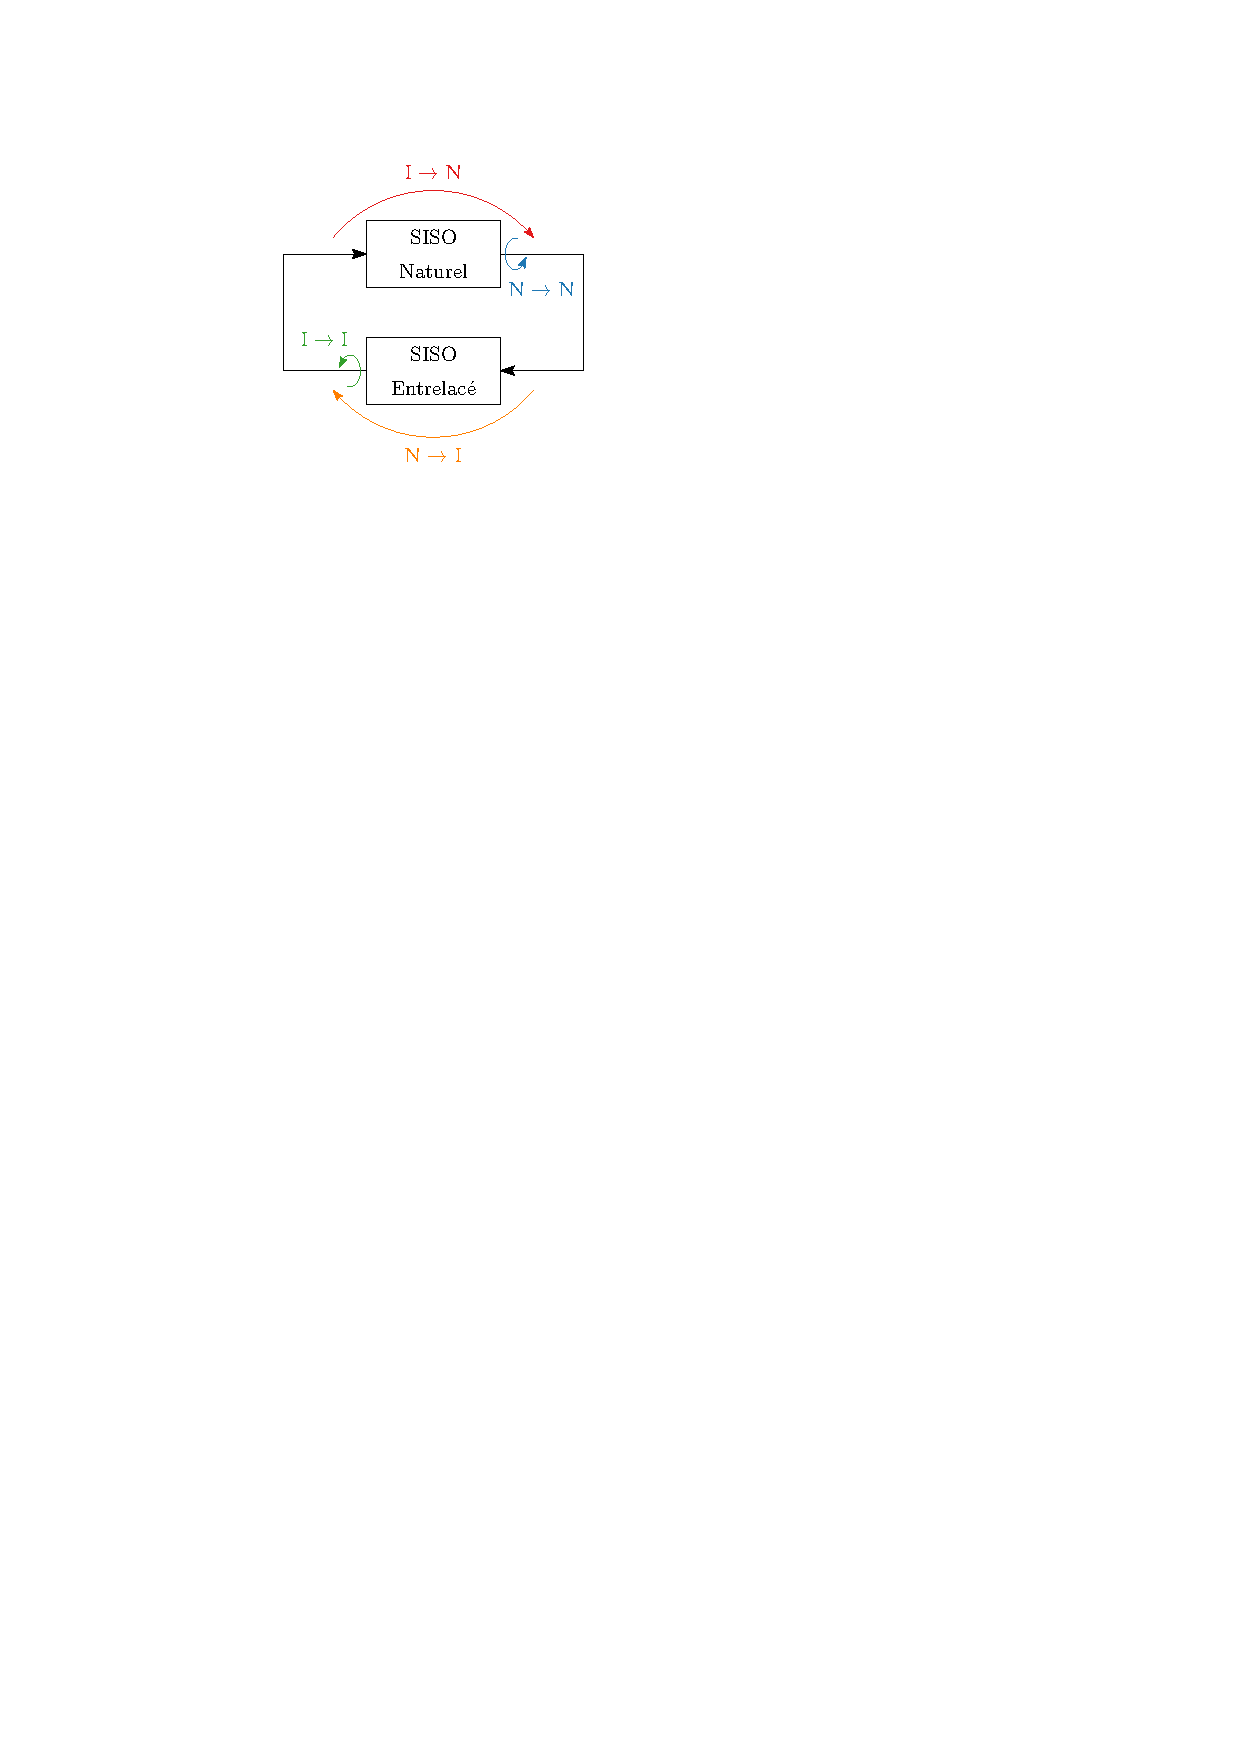
\includegraphics[width=6.5cm]{main/ch2_fig/ipe/osc.pdf}
	\caption{\label{fig:osc}Les différents types d'oscillations possibles pour l'information extrinsèque.}
\end{figure}

Des statistiques quant à l’occurrence de ces quatre types d'oscillations au cours du processus itératif vont maintenant être 
présentées. Celles-ci sont obtenues, dans un premier temps, dans le contexte du turbo code du standard LTE.
Plusieurs valeurs de SNR sont considérés afin d'analyser les oscillations suivant le contexte de fonctionnement du 
décodeur itératif (zones de non-convergence, de convergence et de plancher d'erreurs). Pour toutes ces statistiques, les 
trames considérées sont au nombre de 100. Tout d'abord l'étude sera statique : les moyennes et distribution des 
oscillations par bits seront présentés. Dans un second temps, l'étude sera dynamique en considérant l'évolution des 
oscillations au cours su processus itératif.

\subsection{Turbo codes du standard LTE}
\subsubsection{Nombre moyen d'oscillations par bit}
La première statistique qui peut être obtenue aisément est le nombre moyen d'oscillations par bits. Les bits peuvent être 
répartis selon deux groupes principaux :
\begin{itemize}
	\item bits appartenant à une trame corrigée à la dernière itération,
	\item bits appartenant à une trame erronée à la dernière itération.\newline
\end{itemize}
Ensuite, le second groupe peut lui-même être subdivisé :
\begin{itemize}
	\item bits corrects à la dernière itération dans une trame erronée à la dernière itération,
	\item bits erronés à la dernière itération dans une trame erronée à la dernière itération. \newline
\end{itemize}
La Figure \ref{ch2:fig:meanlte} présente l'évolution du nombre d'oscillations par bit selon la classification qui 
vient d'être introduite et ce, en fonction de la diminution du taux d'erreur trame pour le standard LTE. Le turbo code 
considéré a une taille de trame de 1024 bits d'information pour un rendement 1/3. La sous-figure 
(a) correspond à la zone de non-convergence, les sous-figures (b) et (c) à la zone de convergence et finalement la (d) à 
la zone du plancher d'erreur. Plusieurs constations notables peuvent en être extraites. 

Tout d'abord, le nombre moyen d'oscillations est le même que nous considérions comme référence le décodeur opérant dans le 
domaine naturel ou celui opérant le domaine entrelacé. Ainsi, dans la suite, uniquement les oscillations $N\rightarrow N$ 
et $N\rightarrow I$ seront détaillées dans la suite des analyses.
De plus, quelque soit la valeur du SNR, les informations extrinsèques d'une trame corrigée n'oscillent pas ou très 
peu. En comparaison, les informations extrinsèques d'une trame erronée oscillent quant à elles environ dix fois plus.
Cette constatation est le principe fondamental sur lequel reposent les critères d'arrêts SCR et SDR. En effet, le nombre 
d'oscillations permet d'estimer si une trame a convergé ou non.

\begin{figure}[tb]
	\begin{center}
	\includegraphics[width=.9\textwidth]{main/ch2_fig/tikz/m_lte.pdf}
	\caption{Nombre moyen d'oscillations pour différents taux d'erreurs trame cibles, turbo code du standard LTE (K=1024, R=1/3) \label{ch2:fig:meanlte}}
	\end{center}
\end{figure}

Toujours à partir de la Figure \ref{ch2:fig:meanlte}, en considérant uniquement les trames erronées, il est notable que le nombre moyen 
d’oscillations par bits (tous bits confondus) est très proche du nombre moyen d’oscillations par bits corrigés. Ceci 
provient du fait que le nombre de bits erronés par trame erronée (BE/FE) est relativement faible. En effet, ce dernier 
est largement inférieur à 100 dans la zone de convergence. Il est inférieur à 10 dans la zone du plancher d'erreur. Cela
signifie que dans une trame erronée, la majorité des bits est corrigé. 

Il est encore plus remarquable que les bits erronés oscillent plus que les bits corrigés. Plus la valeur de SNR augmente, 
plus cette constatation est vérifiée. Nous pouvons constater sur la Figure \ref{ch2:fig:meanlte} que les bits erronées 
oscillent environ dix fois pour l'oscillation $N\rightarrow N$ et environ seize fois pour 
l'oscillation $N\rightarrow I$, ce quelque soit la valeur du SNR. En revanche, le nombre moyen d'oscillations des bits corrigés 
diminue graduellement lorsque la valeur de SNR augmente. Ainsi, au sein des trames erronées, au niveau du plancher d'erreur 
du turbo code du standard LTE, les bits erronés oscillent quatre fois plus que les bits corrigés.

Pour conclure les observations résultant de la Figure \ref{ch2:fig:meanlte}, pour une raison de symétrie dans l'architecture 
du décodeur, le nombre d'oscillations par bit est lui aussi symétrique vis-à-vis de l'entrelaceur. Ainsi, seuls deux types 
d'oscillations peuvent être considérées dans l'étude. Le nombre d’oscillation par bit est un critère discriminant les trames 
corrigées. Ceci a permis la définition des critères d'arrêts SDR et SCR. Plus encore, si un bit est erroné, alors, en moyenne, 
il aura plus oscillé que les bits corrigés. Cependant, pour pouvoir améliorer le processus de décodage, il est intéressant 
d'essayer d'établir si la réciproque est vraie : 
\og Si un bit a oscillé plus que la moyenne, alors il est erroné \fg. Pour répondre à cette question, les statistiques doivent
être présentées selon une granularité différente : celles-ci se doivent d'être présentés au niveau trame.

\subsubsection{Comportement des oscillations au niveau trame au cours du processus itératif} 
Dans cette partie, les oscillations sont présentées au cours du processus itératif. Le turbo code du standard LTE avec 
comme paramètres K=1024 et R=1/3 est toujours employé. Seules deux valeurs de SNR sont considérées afin d'en faciliter 
l'analyse. La première correspond à un taux d'erreur trame de $10^{-2}$, donc au début de la zone de convergence. La valeur 
de SNR associée vaut 0,65 dB. La seconde correspond à un taux d'erreur trame de $10^{-5}$, situant les performances de 
décodage dans la zone du plancher d'erreur. La valeur de SNR associée vaut 1,2 dB.

\begin{figure}[!ht]
	\hspace*{-.7cm}
	\begin{center}
	\includegraphics[width=.9\textwidth]{main/ch2_fig/tikz/it_lte10-2.pdf}
	\caption{Oscillations au cours des itérations dans le cadre du standard LTE (K=1024, R=1/3) pour un taux d'erreur trame de $10^{-2}$ \label{ch2:fig:it_lte_1}}
	\end{center}
\end{figure}

Les résultats pour un taux d'erreur trame de $10^{-2}$ sont présentés dans la  Figure \ref{ch2:fig:it_lte_1}. Cette 
Figure est divisée en six sous-figures. La première colonne traite des trames erronées à l'issue du processus 
itératif. La seconde colonne concerne les trames corrigées. Deux types d'oscillations sont présentées : le nombre d'oscillations 
$N\rightarrow N$, le nombre d'oscillations $N\rightarrow I$. Conjointement à ceci, le nombre d'erreurs associé est aussi 
présenté.

Nous pouvons remarquer que les trames corrigées à la 32\textsuperscript{ème} itération alors qu'elles ne l'étaient pas à 
l'issue de la 10\textsuperscript{ème} itération sont marginales. Ceci est à corroborer avec le choix réalisé dans la majorité des 
architectures de turbo décodeur de fixer le nombre maximal d'itérations à moins de 10.
Il est aussi remarquable que le nombre d'erreurs semble être fortement corrélé avec le nombre d'oscillations. En effet, 
les rares trames erronées n'oscillant que peu sont celles qui ne possèdent que peu d'erreurs. Plus généralement,
le nombre d'oscillations semble correspondre au double du nombre d'erreurs.

La Figure \ref{ch2:fig:it_lte_2} détaille le même type d'information que la Figure \ref{ch2:fig:it_lte_1} mais pour un 
taux d'erreur trame cible de $10^{-5}$. Pour le standard LTE, ceci correspond à un fonctionnement du 
turbo décodeur au début du plancher d'erreur. Nous pouvons remarquer que pour les trames corrigées, la convergence est 
plus rapide : seulement quelques itérations sont nécessaires. Pour les trames erronées à l'issue 
du processus itératif, des trames possédant un nombre important d'erreurs sont rares. Elles correspondent à celles 
présentant le plus grand nombre d'oscillations. De fait, la majorité des trames erronées possèdent un faible nombre 
d'erreurs. Ces dernières sont majoritairement constantes après la cinquième itération.

Finalement, ces nouvelles observations permettent de mieux analyser les oscillations durant le processus itératif. Il est alors 
notable que d'une part, pour les trames erronées, deux \og modes \fg ~d'oscillations sont visibles :
\begin{itemize}
	\item le nombre d'oscillations est très important. Des variations sont observées au cours des itérations mais elles 
	restent dans la plage de valeurs $[200,400]$.
	\item le nombre d'oscillations est faible et varie peu.
\end{itemize}

D'autre part, une corrélation forte entre le nombre d'erreurs et le nombre d'oscillations a été constaté. Cependant 
cette analyse a été menée au niveau trame. Il est donc maintenant nécessaire de descendre de niveau de granularité pour observer 
la distribution des oscillations au sein des trames erronées.

\begin{figure}[!t]
	\hspace*{-.7cm}
	\begin{center}
	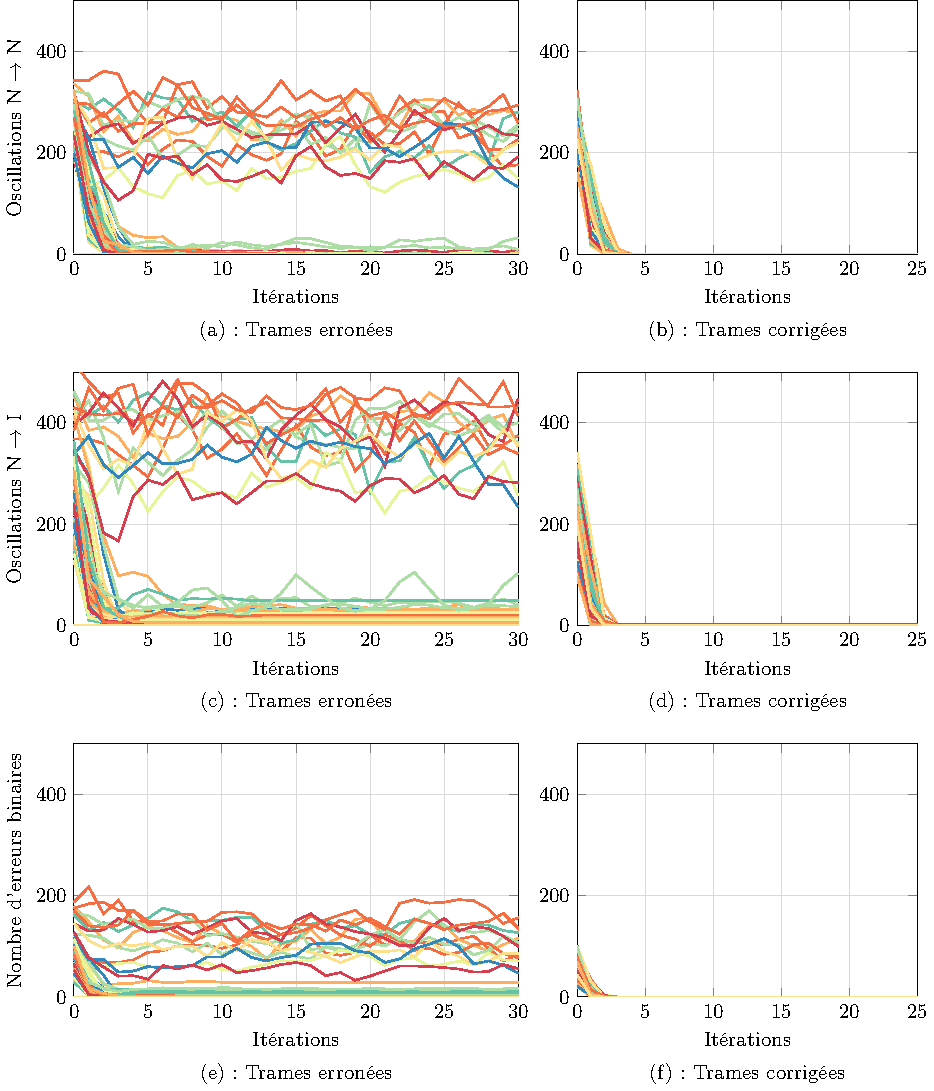
\includegraphics[width=.9\textwidth]{main/ch2_fig/tikz/it_lte10-5.pdf}
	\caption{Oscillations au cours du processus itératif dans le cadre du standard LTE (K=1024, R=1/3) pour un taux d'erreur trame de $10^{-5}$ 
	\label{ch2:fig:it_lte_2}}
	\end{center}
\end{figure}

\subsubsection{Distributions des oscillations au sein des trames erronées} 
Dans cette section, la distribution des oscillations dans les trames erronées est analysée. Dans les sections précédentes,
il a été montré que les bits erronés d'une trame erronée oscillent plus que les bits corrects. La présente analyse permet
d'établir si la réciproque est vraie. Pour ce faire, la Figure \ref{fig:d_lte_10-2} présente l’occurrence du nombre d'oscillations par bit pour un taux 
d'erreur trame cible de $10^{-2}$. Cette Figure, composée de deux histogrammes, considère d'abord les oscillations $N\rightarrow N$ et 
$I\rightarrow I$ (a) puis, les oscillations $N\rightarrow I$ et $I\rightarrow N$ (b). Les occurrences sont normalisées 
par rapport au nombre de bit d'information total par trame.

%À nouveau, le comportement des oscillations est semblable vis-à-vis de la référence (c'est-à-dire que l'on considère 
%$N\rightarrow N$ ou $I\rightarrow I$). 

Dans Figure \ref{fig:d_lte_10-2} (a), $20\%$ des bits sont corrects et n'ont pas oscillé. Il est à noter que 
les nombres d'oscillations impairs sont sous représentés vis-à-vis des nombres d'oscillations pairs. Il semblerait que, 
majoritairement, la première décision prise par un décodeur SISO soit la bonne. Néanmoins, nous n'avons pu tirer d'analyse 
plus conséquente de 
cette observation. La distribution des oscillations des bits erronés est, quand à elle, relativement équirépartie. 

Les oscillations $N\rightarrow I$ et $I\rightarrow N$ ne présentent pas d’irrégularité comme constatée dans les cas 
$N\rightarrow N$ et $I\rightarrow I$. L'allure de la distribution des oscillations pour les bits corrects à l'issu du 
processus itératif semble être l'association de deux gaussiennes : l'une centrée autour de $0$ oscillation et l'autre 
autour de $14$ oscillations. Pour les 
bits erronés, l'allure des distributions est également de forme gaussienne et centrée autour de $16$ oscillations. Cette allure sont à
mettre en corrélation avec le bruit additif lui-même gaussien utilisé sur le canal.

Pour le taux d'erreur trame considéré dans cette analyse, le nombre moyen de bit erroné par trame erroné (BE/FE) vaut 
113. Cela signifie (en considérant la taille de la trame, à savoir 1024) que $11\%$ des bits sont erronées dans une trame erronée. 
Si le nombre d'oscillations est pris en considération, alors la probabilité de bit erroné varie de $0,1\%$ à $19,9\%$. 
Pour les bits oscillant moins de 11 fois, cette probabilité est inférieure à la probabilité moyenne. Par contre, elle
est supérieure à la probabilité moyenne si le bit considéré a oscillé 11 fois ou plus. Ainsi, en considérant les bits 
ayant oscillé 15 fois ou plus, la probabilité qu'ils soient erronés vaut $18\%$. La probabilité d'obtenir un bit 
erroné a alors quasiment doublé. Ces observations sont formalisées dans les équations suivantes :
\[P_{i \in K} (\textnormal{bit } i \textnormal{ est en erreur}) = 11 \%\]
\[P_{i \in K} (\textnormal{bit } i \textnormal{ est en erreur}\ |\ \textnormal{OSC}(i) > 15 ) = 18 \%.\]
Néanmoins, les bits erronés oscillent eux aussi. De plus, comme ils sont majoritaires, il n'existe pas de 
nombre d'oscillations permettant d'obtenir une probabilité d'obtenir un bit erroné supérieure à celle d'obtenir un bit
correct. C'est à dire qu'il n'existe pas $n$ tel que : 
\[P_{i \in K} (\textnormal{bit } i \textnormal{ est en erreur}\ |\ \textnormal{OSC}(i) > n ) > 50 \%.\]


\begin{figure}[!t]
	\centering
	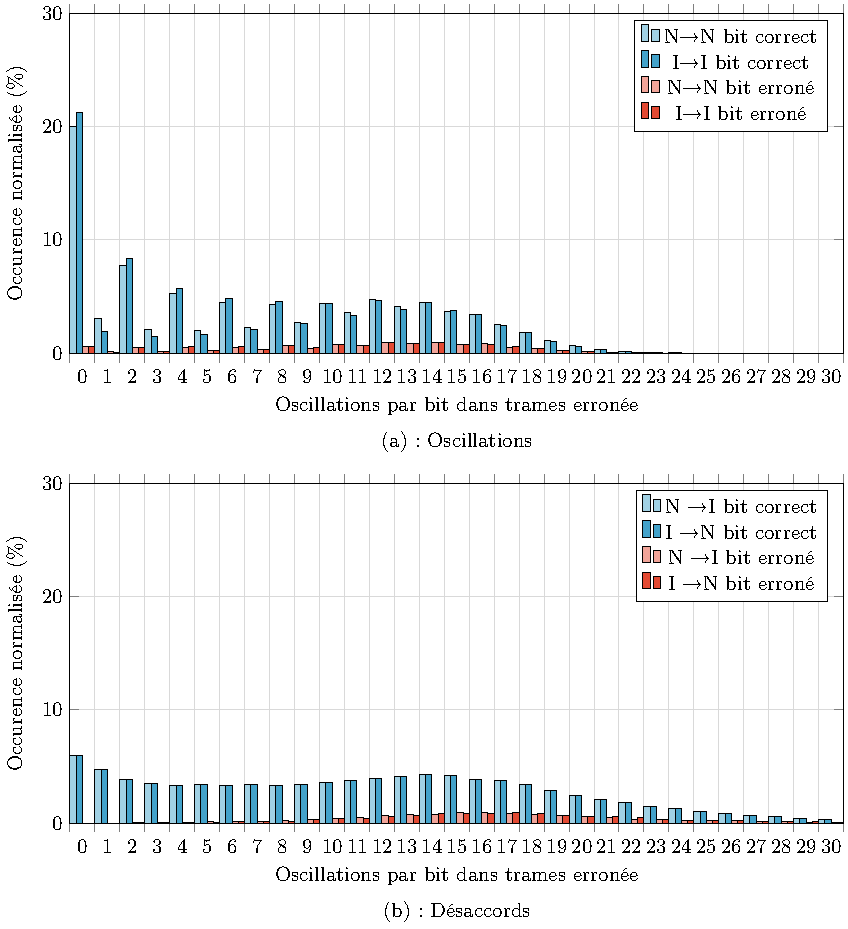
\includegraphics[width=.8\textwidth]{main/ch2_fig/tikz/d_lte_10-2.pdf}
	\caption{Distribution du nombre d'oscillations par bit pour un taux d'erreur trame de $10^{-2}$, pour le turbo code du standard LTE (K=1024, R=1/3) \label{fig:d_lte_10-2}}
\end{figure}

La distribution des oscillations est maintenant présentée en Figure \ref{fig:d_lte_10-5} pour un  taux d'erreur trame 
cible de $10^{-5}$. De part la rapidité de convergence, une seule gaussienne est maintenant visible : celle centrée autour 
de 0 oscillations. 
La seconde gaussienne disparaît progressivement au fur et à mesure que la valeur de SNR augmente. Jusqu'à ce qu'elle ne 
soit plus visible lorsque la valeur de SNR correspond à une position dans le plancher d'erreur.
%Ainsi, par exemple, $70\%$ des bits n'ont pas oscillé dans le sens $N\rightarrow I$ et sont corrects.

Dans le cas considéré, ramené en pourcentage, le taux de bit erroné par trame erronée vaut $1,5\%$. Dès qu'un bit oscille plus de quatre fois, 
le taux de bit erroné par trame erronée est supérieur à ce taux moyen. Plus encore, un bit ayant oscillé plus de 8 fois a une probabilité de $15\%$
d'être erroné. Ce qui formalisé donne :
\[P_{i \in K} (\textnormal{bit } i \textnormal{ est en erreur}) = 0,15 \%\]
\[P_{i \in K} (\textnormal{bit } i \textnormal{ est en erreur}\ |\ \textnormal{OSC}(i) > 8 ) = 15 \%.\]
Cette probabilité est donc multipliée par un facteur 10. Néanmoins, même dans le cas d'un positionnement 
dans le plancher d'erreur, un bit ayant fortement oscillé a plus de chance d'être corrigé que d'être erroné quelque soit le nombre
d'oscillations observés.

\begin{figure}[!t]
	\centering
	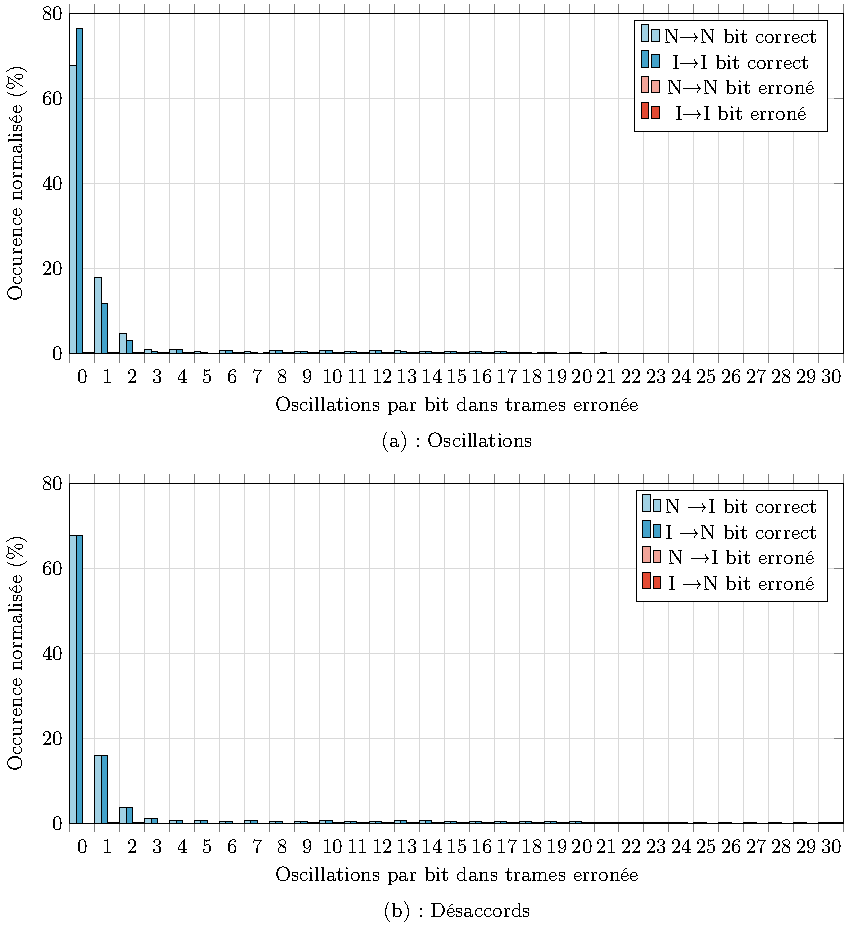
\includegraphics[width=.8\textwidth]{main/ch2_fig/tikz/d_lte_10-5.pdf}
	\caption{Distribution du nombre d'oscillations par bit pour un taux d'erreur trame de $10^{-5}$, pour le standard LTE (K=1024, R=1/3) \label{fig:d_lte_10-5}}
\end{figure}

\subsection{Turbo codes du standard CCSDS}
La même étude à été menée dans le cadre du standard CCSDS. Un rendement de 1/3 est toujours considéré. En revanche, le nombre 
de bits d'information est quant à lui fixé à 1784. Pour faciliter la lecture de l'analyse comparée des résultats suivante, 
les visualisations graphiques de ces statistiques sont déportées en Annexe \ref{sec:annCCSDS}.
\paragraph*{Nombre moyen d'oscillation par bit : } 
Tout d'abord les bits erronées oscillent légèrement plus dans le contexte CCSDS que dans le contexte LTE. En effet, 
quelque soit la valeur de SNR, 12 oscillations $N\rightarrow N$ et 16 oscillations $N\rightarrow I$ sont observées. Elles 
s'établissaient respectivement à 10 et 15 pour le turbo code du standard LTE. Les nombres d'oscillations des bits corrigés diminuent quant à eux
avec l’augmentation de la valeur de SNR. Cependant, plus que de la valeur du taux d'erreur trame ou de la valeur de SNR,
c'est la position dans la courbe de performance qui dicte ce phénomène. Par exemple, le ratio entre le nombre 
d'oscillations pour les bit erronés et les bits corrects au sein des trames erronées vaut 1,7 pour le turbo code du 
standard CCSDS fonctionnant à un taux d'erreur trame de $10^{-6}$. Ce dernier est de 1,9 pour le turbo code du 
standard LTE fonctionnant à un taux d'erreur trame de $10^{-4}$. Ainsi, deux ordres de magnitude séparent ces deux mesures,
bien qu'elles correspondent toutes deux à un fonctionnement peu avant la zone du plancher d'erreur, assurant des statistiques similaires.
\paragraph*{Comportement des oscillations au cours du processus  : }
Pour de faibles valeurs de SNR, le turbo code du standard CCSDS requiert quelques itérations supplémentaires pour converger en comparaison de son homologue
LTE. Cette constatation peut être imputée à l'augmentation de la longueur de contrainte entre les deux turbo codes. Néanmoins,
la grande majorité des trames est encore corrigée en moins de 10 itérations. À nouveau, une forte corrélation apparaît 
entre le nombre d'oscillations et le nombre d'erreurs. Ainsi, le nombre d'erreurs est proche de la moitié du nombre d'oscillations
$N \rightarrow N$. Le nombre d'erreurs est plus important dans le cas du turbo code du standard CCSDS. Mais cette hausse est
directement liée aux tailles de trames considérées, à savoir plus importante pour le turbo code du standard CCSDS.\\
Lorsque la valeur de SNR augmente, le même comportement que celui décrit précédemment pour le turbo code du standard LTE apparaît. 
Moins d'itérations sont nécessaires pour corriger les trames et une grande part des trames erronées à l'issu du processus de décodage 
n'a que peu d'erreurs binaires. Néanmoins, à fort SNR, une plus grande démarcation est visible entre les trames erronées 
avec peu d'erreurs et celles contenant un nombre importants d'erreurs.
\paragraph*{Distribution des oscillations au sein des trames erronées : }
En ce qui concerne la dernière statistique, le constat est similaire. Pour un  taux d'erreur trame 
cible de $6\times 10^{-7}$, le taux de bit erroné par trame erronée, ramené en pourcentage, vaut $3,1\%$. La probabilité
d'obtenir un bit erroné est supérieur à ce taux dès que le bit considéré a oscillé plus de 6 fois. Plus encore, un bit 
ayant oscillé plus de 11 fois a une probabilité de $16\%$ d'être erroné. Ce qui formalisé donne :
\[P_{i \in K} (\textnormal{bit } i \textnormal{ est en erreur}) = 3,1 \%\]
\[P_{i \in K} (\textnormal{bit } i \textnormal{ est en erreur}\ |\ \textnormal{OSC}(i) \geq 11 ) = 16 \%.\] 
Ainsi, la probabilité de choisir un bit erroné a crû d'un facteur 5. 

Finalement, les observations réalisées dans le cadre du turbo code du standard CCSDS sont similaires à celles obtenues avec
le turbo code du standard LTE. Le paragraphe suivant récapitule ces résultats et conclut cette section.

\subsection{Analyse globale et conclusions}
De ces différentes observations statistiques, plusieurs constats peuvent être énoncés.
\begin{enumerate}
\item Tout d'abord, il a été noté que si des oscillations surviennent lors d'une itération, alors la trame n'est pas encore 
corrigée. 
\item De plus, une corrélation forte entre le nombre d'erreurs et le nombre d'oscillations a été mis en évidence. 
\item De fait, plus que du nombre d'états du codeur ou de l'entrelaceur, c'est du régime de fonctionnement du turbo décodeur que dépend
le nombre d'oscillations et la distribution de ces oscillations.
\item Si un bit oscille fortement, alors, relativement aux autres, il a plus de chance d'être erroné.
\item Ainsi, c'est parmi les bits oscillant le plus que se trouve la plupart des bits erronés.
\item Cependant, comme les bits corrigés à l'issu du processus itératif oscillent eux aussi et sont majoritaires dans la 
trame, le nombre d'oscillation ne permet pas de prédire si un bit est erroné.
\end{enumerate}

En conclusion, l'observation des oscillations ne semble pas pouvoir permettre de proposer une méthode directe au sein du 
turbo décodage permettant l'amélioration des performances des turbo codes. Cependant, de part la forte corrélation entre 
le nombre d'erreurs et le nombre d'oscillations, une modification du décodage EML-MAP exploitant les oscillations est décrite 
dans la section suivante.
%%%%%%%%%%%%%%%%%%%%%%%%%%%%%%%%%%%%%%%%%%%%%%%%%%%%
\section{L’algorithme Self-Corrected EML-MAP}
En 2008, V. Savin  a proposé une modification de l'algorithme Min-Sum \cite{wiberg1996codes} pour le décodage des codes 
LDPC permettant d'approcher les performances de l'algorithme Sum-Product \cite{wiberg1996codes}. Cet algorithme de 
décodage est nommé Self-Corrected Min-Sum \cite{savin_sc}.

Dans un premier temps, le principe de cet algorithme est présenté pour le décodage des codes LDPC. Ensuite, une 
adaptation pour le décodage des turbo codes est proposée. Les performances de ce nouvel algorithme seront alors détaillées.

\subsection{La méthode originelle pour les codes LDPC}
Le décodage des codes LDPC, comme le décodage des turbo codes repose sur un processus itératif. Pour les codes LDPC,
chaque itération est composée de trois étapes : 
\begin{enumerate}
	\item Calcul des nœuds de parité ($\beta$),
	\item Calcul des nœuds de variable ($\alpha$).
	\item Calcul de l'information \textit{a posteriori} ($\gamma$),
\end{enumerate}
Le principe du Self-Corrected est de détecter les messages non fiables échangés lors du décodage itératif et de les \og 
effacer \fg. Cela correspond à fixer à 0 les valeurs LLRs associées à ces messages. Ainsi, la valeur d'un nœud de 
variables ($\alpha$) est effacée si son signe a changé par rapport à l’itération précédente. Dans le cas contraire, sa 
valeur est transmise, sans modification, aux nœuds de 
parité. De la sorte, le décodeur détecte les messages non fiables et les écarte du processus de décodage. Hormis cette 
étape, les autres étapes de cet algorithme sont les mêmes que celles d'un algorithme de propagation de croyance.

Finalement, l'algorithme Self-Corrected permet d'approcher les performances de l'algorithme Sum-Product dans la zone de convergence alors
que ce dernier possède une complexité calculatoire bien plus importante. Pis encore, dans certains contextes, il peut même le 
surpasser dans la zone du plancher d'erreur.

\subsection{Adaptation aux turbo codes binaires}
La transposition du Self-Corrected Min-Sum au décodage des turbo codes est relativement aisée. En effet, les messages provenant 
des nœuds de variable à destination des nœuds de parité correspondent aux informations extrinsèques échangées lors 
du processus itératif de décodage de turbo code.

Ainsi, la remise à zéro peut être effectuée lorsqu'une oscillation $N \rightarrow N$ ou $I \rightarrow I$ est détectée.
L'Algorithme \ref{alg:sc1} détaille cette adaptation pour le décodage des turbo codes. Le principe de cette approche est 
donc le suivant : si l’information extrinsèque calculée par un décodeur SISO pour un bit de la trame change de 
signe d’une itération à la suivante, alors, celle-ci est remise à zéro avant qu’elle ne soit transmise à l’autre 
décodeur SISO.

Il est à noter que cette adaptation de l'information extrinsèque ne doit pas être appliquée dès la première itération 
du processus de décodage. En effet, dans ce cas, l’intérêt du processus itératif du turbo décodage se verrait annihilé par l'approche Self-Corrected.
Une dégradation des performances vis-à-vis de celles obtenues avec l'algorithme EML-MAP simple serait alors observée.
Il est donc préférable de laisser l'algorithme EML-MAP converger durant les premières itérations et ensuite d'appliquer le principe 
Self-Corrected (SC). À l'aide de simulations Monte-Carlo, il a été montré que le nombre d'itérations sans SC doit être 
choisi entre 3 et 5 pour obtenir les meilleures performances de décodage. Ces dernières sont présentées en section suivante.
Dans la suite, le principe SC est appliqué à partir de la quatrième itération.

\begin{center}
\begin{minipage}{.6\textwidth}%
%\vspace*{-.8cm}
% \begin{algorithm}[H]
% \caption{: Self-Corrected EML-MAP}
% \label{alg:sc1}
% \begin{algorithmic}
% \For{\emph{j} de 0 \`a it\'eration maximum}
% \State \Call{Décodage SISO$_1$ EML-MAP}{}
% %\State $\mathbf{L_{12}^{\texttt{e}\ (j)}} \gets \mathbf{L_{12}^{\texttt{e}\ (j)}}\times 0.75 $
% \If {$j>4$} \textbf{pour tout} k
% \If {$sgn(\mathbf{L_{12}^{\texttt{e}\ (j)}}(k)) \neq sgn(\mathbf{L_{12}^{\texttt{e}\ (j-1)}}(k))$}
% \State {$\mathbf{L_{12}^{\texttt{e}\ (j)}}(k)\gets 0$}
% \EndIf
% \EndIf
% \State \Call{Décodage SISO$_2$ EML-MAP}{}
% %\State $\mathbf{L_{21}^{\texttt{e}\ (j)}} \gets \mathbf{L_{21}^{\texttt{e}\ (j)}}\times 0.75 $
% \If {$j>3$} \textbf{pour tout} k
% \If {$sgn(\mathbf{L_{21}^{\texttt{e}\ (j)}}(k)) \neq sgn(\mathbf{L_{21}^{\texttt{e}\ (j-1)}}(k))$}
% \State {$\mathbf{L_{21}^{\texttt{e}\ (j)}}(k)\gets 0$}
% \EndIf
% \EndIf
% % \If {$j>3$ \textbf{et} CRC v\'erifi\'e}
% % \State \Call{Sortie boucle}{}
% % \EndIf
% \EndFor
% \end{algorithmic}
% \end{algorithm}
	\begin{algorithm}[H]
		\DontPrintSemicolon
		%\KwResult{Write here the result }
		\SetKwFunction{DA}{Décodage SISO$_1$ EML-MAP}
		\SetKwFunction{DB}{Décodage SISO$_2$ EML-MAP}
		
		\For{i: 1 to  $I_{max}$}
		{
			\DA\;
			\If{j>4}
			{
				\ForEach{$k \in K$}{%
					\If{$sgn\left(\mathbf{L_{12}^{\texttt{e}\ (j)}}(k)\right) \neq sgn\left(\mathbf{L_{12}^{\texttt{e}\ (j-1)}}(k)\right)$}
					{
						{$\mathbf{L_{12}^{\texttt{e}\ (j)}}(k)\gets 0$}
					}
				}
			}
			\DB\;
			\If{j>4}
			{
				\ForEach{$k \in K$}{%
					\If{$sgn\left(\mathbf{L_{21}^{\texttt{e}\ (j)}}(k)\right) \neq sgn\left(\mathbf{L_{21}^{\texttt{e}\ (j-1)}}(k)\right)$}
					{
						{$\mathbf{L_{21}^{\texttt{e}\ (j)}}(k)\gets 0$}
					}
				}
			}
		}
	\caption{: Self-Corrected EML-MAP}
	\label{alg:sc1}
	\end{algorithm}
\end{minipage}
\end{center}

\subsection{Performances du principe SC appliqué aux turbo codes binaires}
Cette section présente les performances de décodage obtenues avec l'algorithme Self-Corrected. Dans un premier temps, 
l'étude est menée en considérant un entrelaceur uniforme. Dans un second temps, un cas concret de turbo codes standardisé est considéré.
\subsubsection{Entrelaceur uniforme}
Comme présenté en section \ref{sec:entrelacement}, l'entrelaceur uniforme permet d'extraire les paramètres des codes 
constituant un turbo code. Il permet aussi de décorréler l'impact de l'étape d'entrelacement des performances de 
décodage. 

L'étude est menée sur des turbo codes binaires à 8, 16 et 32 états. Pour les deux premiers, le codeur du standard LTE
et celui du standard CCSDS sont respectivement considérés. Leurs générateurs en octal sont $\{13,15\}$ et $\{23,33\}$. Le 
turbo code à 32 états présentant les meilleures propriétés de distance a quant à lui pour générateur $\{43,63\}$. C'est 
celui-ci que nous avons retenu.

La Figure \ref{fig:sc8it} présente à la fois le taux d'erreur binaire et le taux d'erreur trame pour les trois turbo 
codes sus-mentionnés. La trame traitée par le turbo codeur se compose de 1504 bits. Le décodage est réalisé par
l'algorithme EML-MAP ou par l’algorithme Self-Corrected EML-MAP.
Dans les deux cas, le facteur de remise à l'échelle des informations extrinsèques vaut $0,75$ tout au long du processus itératif.
Le nombre maximal d'itérations est fixé à 8. Un critère d'arrêt basé sur un CRC de 24 bits est utilisé afin de réduire le
temps de simulation.

\begin{figure}[!ht]
	\vspace*{-.2cm}
	\centering
	\includegraphics[width=.8\textwidth]{main/ch2_fig/tikz/sc_8it.pdf}
	\vspace*{-.1cm}
	\caption{Comparaison des performances de décodage entre l'algorithme EML-MAP et l'algorithme SC EML-MAP, 8 itérations au maximum, $K=1504$, $R=\frac{1}{3}$. \label{fig:sc8it}}
	\vspace*{-.1cm}
\end{figure}

Au niveau du taux d'erreur trame, nous pouvons remarquer que l'algorithme SC a des performances moindres que celles de
l'algorithme EML-MAP pour un turbo code à 8 états. Pour le un turbo code à 16 états, les performances sont équivalentes. 
Enfin, pour le turbo code à 32 états, un léger gain apparaît en faveur de l'algorithme SC.
En revanche, quant au taux d'erreur binaire, des gains apparaissent pour les turbo codes à 16 et à 32 états. Les performances 
sont les mêmes pour le turbo code à 8 états.

Ainsi, dans tous les cas, le nombre de bits erronés par trame erronée est réduit via l'adjonction \og d'effacements \fg 
de l'information extrinsèque. En réduisant les oscillations au cours du processus itératif, mais sans néanmoins les inhiber,
le nombre d'erreurs est diminué. Un impact important quant à la longueur de contrainte du codeur élémentaire apparaît :
la correction apporte des gains lorsque la longueur de contrainte augmente. La sous-optimalité du décodage est donc légèrement réduite. 
%TODO: Réflexion nb branches, impact stabilité de la valeur

\begin{figure}[!ht]
\vspace*{-.2cm}
	\centering
	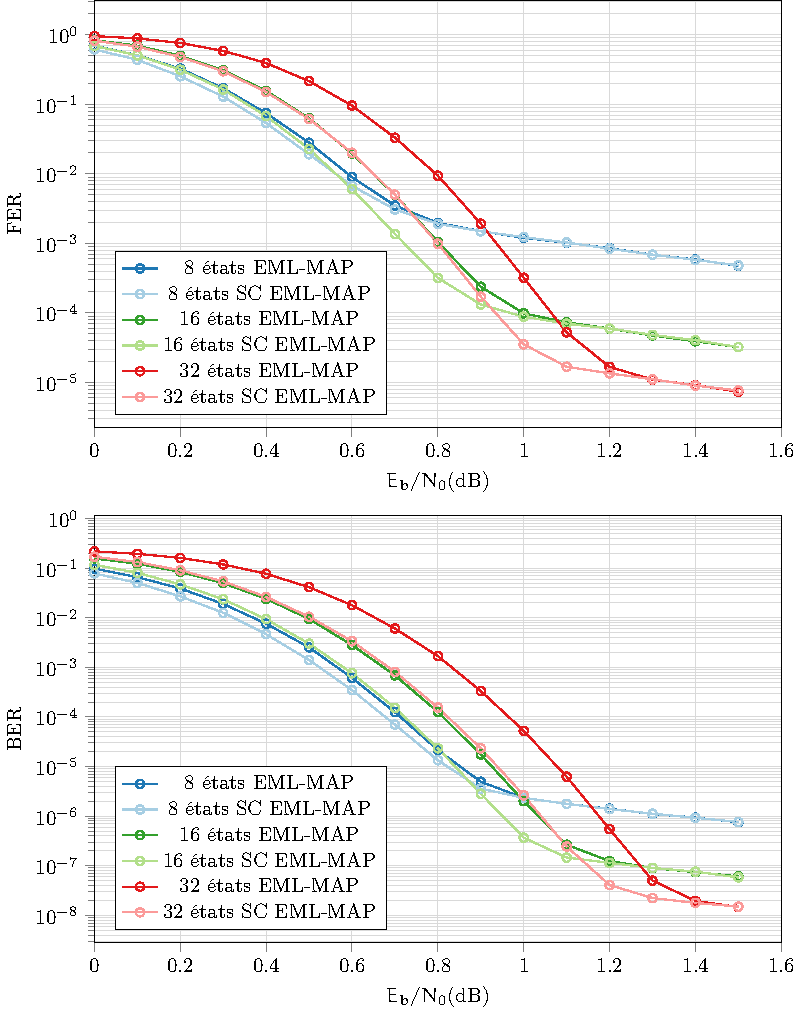
\includegraphics[width=.8\textwidth]{main/ch2_fig/tikz/sc_32it.pdf}
	\caption{Comparaison des performances de décodage entre l'algorithme EML-MAP et l'algorithme SC EML-MAP, 32 itérations au maximum, $K=1504$, $R=\frac{1}{3}$.\label{fig:sc32it}}
\vspace*{-2ex}
\end{figure}

La Figure \ref{fig:sc32it} reprend la même étude mais en fixant cette fois le nombre maximal d'itérations à 32. Maintenant,
quelque soit le nombre d'états, des gains sont obtenus à la fois en terme de taux d'erreur trame et en taux d'erreur binaire.\\
Dans les deux cas, nous pouvons montrer que le taux d'erreur dans le zone de convergence est équivalent entre un turbo code de  
longueur de contrainte $L$ décodé via l'algorithme EML-MAP itérant 32 fois et un turbo code de longueur de contrainte 
$2\times L$ décodé via l'algorithme SC EML-MAP itérant 32 fois. En résumé, en utilisant un entrelaceur uniforme et en 
fixant le nombre maximal d'itérations à 32, les gains obtenus dans la zone de convergence en utilisant l'algorithme SC 
EML-MAP à la place de l'algorithme EML-MAP correspondent à :
\begin{itemize}
	\item $0,02$ dB pour un turbo code à 8 états,
	\item $0,1$ dB pour un turbo code à 16 états,
	\item $0,15$ dB pour un turbo code à 32 états. \\
\end{itemize}

Comme présenté en Chapitre 1, l'augmentation de la longueur de contrainte permet une hausse de la distance minimale du code.
Cela permet donc d'abaisser le plancher d'erreur d'un turbo code. Cependant, le décalage du seuil de 
convergence inhérent à cette augmentation peut empêcher son choix dans un contexte nécessitant de bonnes performances de 
correction pour de faibles valeurs de SNR. Grâce 
à l’algorithme SC EML-MAP, ce désagrément n’apparaît pas. Il est possible de profiter d'une augmentation de la 
$d_{min}$ du code tout en ne subissant pas l'un des désavantages inhérent.

Dans la section suivante, le turbo code du standard CCSDS est considéré. Ce turbo code possède une longueur de 
contrainte de $5$. Les résultats qui viennent d'être exposés montrent que cette longueur de contrainte est la 
longueur minimale requise afin d'observer des gains notables au niveau performances. 

\subsubsection{Turbo code standardisé}
La Figure \ref{fig:ccsds_sc} présente la comparaison des performances de décodage d'un turbo code du standard CCSDS. 
La taille de la trame considérée est de 1784 bits et le rendement du code vaut $1/3$. Dans ce standard, un code CRC est 
défini en amont du turbo code \cite{ccsdsBluebook}. Ce CRC, nommé CRC-CCITT-16, a pour polynôme générateur $(1021)_{16}$. 
Il a donc une traille de 16. Il est retenu dans la suite comme critère d'arrêt. De part sa faible taille, sa distance 
minimale est elle aussi relativement faible. Afin de ne pas dégrader les performances de décodage provenant d'erreurs 
non détectées par le code CRC, la vérification n'est réalisée qu'à partir de l'itération 4 du processus de turbo décodage.
C'est aussi à partir de cette itération que le principe SC commence à être utilisé.

Dans ce contexte, il apparaît que les gains obtenus grâce au principe Self-Corrected, exprimés en terme de dB, sont similaires à ceux de la 
section précédente. Ainsi, en considérant 32 itérations, les gains correspondent à un ordre de grandeur en 
terme de taux d'erreur trame et de taux d'erreur binaire dans la zone de convergence vis-à-vis de l'algorithme EML-MAP. 
Ils gains permettent d'obtenir les mêmes performances en terme de FER que celles obtenues en considérant l'algorithme 
MAP itérant 10 fois. La complexité calculatoire de l’algorithme MAP 
est largement supérieure à celle de l'algorithme EML-MAP. En effet, ce premier requiert l’emploi de fonctions complexes 
tels que des logarithmes, des exponentielles et des opérations de multiplication. Ainsi, le coût en latence qui est dû 
au triplement du nombre d'itérations nécessaires au bon fonctionnement du SC 
EML-MAP est à mettre en regard de la complexité calculatoire de l'algorithme MAP. 
De plus, grâce à l'utilisation du code CRC comme critère d'arrêt, le nombre moyen d'itérations est largement inférieur à 10. 
Par exemple, pour une valeur de SNR de 1 dB, plus de $99\%$ des trames sont corrigées à la quatrième itération. Celle-ci étant la première 
itération à partir de laquelle le CRC est vérifié. 

Le tableau \ref{tab:itmoy} donne le nombre moyen d'itérations nécessaire au turbo décodeur selon qu'il soit basé sur 
l'algorithme SC EML-MAP ou sur l'algorithme EML-MAP. Dans les deux cas, ces valeurs sont approximativement les mêmes. 
Puisque la contribution de certaines valeurs extrinsèques sont annulées et puisqu'il faut un nombre conséquent d'itérations 
pour observer des gains lors de l'application du SC EML-MAP, il pourrait être attendu que le principe SC ralentisse la vitesse 
de convergence du processus itératif. Cependant, cela n'est pas constaté dans le nombre d'itérations moyen.

En fait, les nombres moyen d'itérations sont proches du nombre moyen d'itérations utilisées lorsqu'un critère d'arrêt 
génie -- c'est-à-dire en connaissant la trame transmise -- est considérée \cite{matache2000stopping}.
\begin{table}[!h]
	\centering
	\renewcommand{\arraystretch}{.9}
	\begin{tabular}{lrrr}
		\toprule
		    & \textbf{EML-MAP} & \textbf{SC EML-MAP} & \textbf{Génie} (\cite{matache2000stopping})\\ 
		 \cmidrule(l){2-2} \cmidrule(l){3-3} \cmidrule(l){4-4} 
		0.6 dB & 5.9 &  5.9 & 4.0\\
		0.8 dB & 4.3 & 4.4 & 3.2\\
		1.0 dB & 4.0 & 4.0 & \\
		\bottomrule
	\end{tabular}
	\caption{Comparaison du nombre moyen d’itérations nécessaires selon l'algorithme de turbo décodage}
	\label{tab:itmoy}
\end{table}

\begin{figure}[tb]
	\centering
	\includegraphics[width=.8\textwidth]{main/ch2_fig/tikz/ccsds_sc.pdf}
	\vspace*{.3cm}
	\caption{\label{fig:ccsds_sc}Comparaison des performances décodage entre les algorithme EML-MAP, SC EML-MAP et MAP. Turbo code du standard CCSDS (K=1784, R=1/3).}
\end{figure}


\subsubsection{Turbo code double binaire}
Des tentatives d'extension du principe Self-Correct de l'information extrinsèque au cas des turbo codes double binaires 
ont été menées. Cependant, lors du décodage d'un tel code, trois valeurs de LRV sont échangées entre les décodeurs 
élémentaires pour un symbole. Chacun de ces LRV représente alors respectivement la probabilité que le symbole 1, le symbole 
2 ou le symbole 3 ait été émis rapporté à la probabilité que le symbole 0 ait été émis. 

Dans le cas binaire, le principe Self-Correct peut être interprété de la sorte : \og lorsqu'un des décodeurs élémentaire 
change d'avis sur la valeur d'un bit d'une itération à l'autre, sa contribution au processus itératif est annulée pour 
le bit considéré \fg. Dans un contexte double binaire, la décision correspond à 0 si les trois LRV sont négatifs et à 
l'index du maximum sinon. Ainsi, l'élément déclencheur de la correction SC peut être le changement de l'index du maximum 
parmi ces trois LRV.

\og L'annulation de la contribution \fg ~dans le cadre binaire ne peut avoir différentes interprétations. En effet, cela 
correspond forcement à passer la valeur du LRV considéré à 0. Ainsi le poids de la probabilité que le bit soit 0 et 
le poids de la probabilité que le bit soit 1 sont les mêmes. En revanche, dans le cas double binaire l'interprétation n'est 
pas aussi triviale, car 4 probabilités sont simultanément considérées. Ainsi, plusieurs interprétations sont possibles. Pour plus 
de clarté, un exemple illustrant ces propositions est présenté dans le tableau \ref{tab:exsc}. L'approche Self-Corrected 
peut donc affecter valeurs des informations extrinsèques en 
\begin{itemize}
	\item les assignant toutes trois à la même valeur (a):
	\begin{itemize}
		\item si la valeur 0 est choisie, alors seul le canal contribue au calcul des métriques de branche,
		\item si une autre valeur est choisie, elle n'aura toute fois pas d'impact en raison de l’opération 
		ACS dans le calcul des métriques de nœud.
	\end{itemize}
	\item en assignant deux à une même valeur et la troisième à une autre. Trois cas sont alors à considérer :
	\begin{itemize}
		\item répétition de la valeur maximale (b),
		\item répétition de la valeur médiane (c),
		\item répétition de la valeur minimale (d) et (e).
	\end{itemize}
	\item usant d'une autre remise à l'échelle (f).
	\item inhibant le calcul nouvellement effectué par le décodeur (g).\\
\end{itemize}

L'ensemble de ces propositions a été mise en œuvre et évalué par des simulations Monte-Carlo. Les turbo codes des standards 
DVB-RCS et DVB-RCS2 ont été considérés. Aucun gain significatif n'a été relevé, quelques soient les rendements de code ou les tailles de 
trames considérés. Dans le meilleur des cas, un gain d'un facteur 2 apparaît en terme de taux d'erreur trame. 

\begin{table}[t]
	\centering
	\begin{tabular}{llrrrrrrr}
		\toprule
		    It n & It n+1 & a & b & c & d &e &f &g\\ 
		 \cmidrule(r){1-1} \cmidrule(r){2-2} \cmidrule(l){3-9} 
		 7 & 6 & 0 & 8 & 6 & 2 & 6 & 6  & 7 \\
		 5 & 8 & 0 & 8 & 6 & 6 & 2 & 4,5 & 5 \\
		 2 & 2 & 0 & 2 & 2 & 2 & 2 & 1,5 & 2 \\
		\bottomrule
	\end{tabular}
	\caption{Exemples des différentes interprétations considérées pour la correction de l'information extrinsèque pour les turbo codes doubles binaires}
	\label{tab:exsc}
\end{table}

Des espoirs résidaient dans le standard DVB-RCS2 puisque ce turbo code double binaire se compose de 16 états, nombre 
d'états permettant l'observation de gains notables dans le cas de turbo codes binaires. Cependant, l'absence de gains 
est sans doute à mettre en corrélation avec la constatation énoncée dans \cite{doublebinadvantages}. Cette dernière
indique que l'un des avantages des turbo codes double binaires vis-à-vis de leurs homologues binaires est le plus faible 
écart au niveau des performances de décodages entre l’algorithme EML-MAP et l'algorithme MAP. Ainsi, dans le cas double 
binaire, la sous optimalité de l'algorithme ML-MAP vis-à-vis de l'algorithme MAP 
est moins important. Les gains pouvant être obtenus par un algorithme visant à corriger la sous optimalité pour de tels 
codes ne peuvent être donc que plus faibles.

À la vue des faibles gains obtenus via cette tentative de transposition, l'étude a été interrompue
pour ce contexte. En section suivante, une étude architecturale portant sur le décodage de turbo codes binaire selon 
l'algorithme SC EML-MAP est menée.

\subsection{Etude architecturale}
Dans cette section, la description d'une architecture matérielle permettant le décodage de turbo codes exploitant le principe 
Self-Corrected de l'information extrinsèque est menée. 

La Figure \ref{fig:sc_arch} présente l'ensemble de l'architecture proposée. Elle a pour base un décodeur ML-MAP séquentiel, 
comme décrit dans \cite{livre_declercq}. Son principe est le suivant. Les 
informations du canal et l'information extrinsèque calculée à la demi-itération précédente sont traités séquentiellement. De 
la première paire de données, les métriques de branche sont calculées. Elles permettent alors de calculer les métriques 
de nœud aller. Parallèlement, les métriques de branche sont mémorisées dans un registre tampon LIFO (Last In First Out ou 
dernier arrivé, premier servi). Une fois les métriques de nœud aller calculées, le calcul des métriques de nœud retour débute. 
Pour la première section de treillis, les métriques de branche, de nœud aller et de nœud retour sont alors calculées. 
Elles sont combinées selon qu'elles correspondent à une transition associée à un 0 émis ou un 1 émis. Le maximum 
correspondant à chacune des transitions est extrait. Ils sont alors soustrait entre eux afin d'obtenir l'information \textit{a posteriori}. N'y reste plus qu'à soustraire l'information provenant du canal et celle calculée à la demi-itération 
précédente pour obtenir l'information extrinsèque. Celle-ci est alors stockée de manière séquentielle en mémoire afin 
de pouvoir être utilisée lors de la demi-itération suivante.

\begin{figure}[!t]
	\centering
	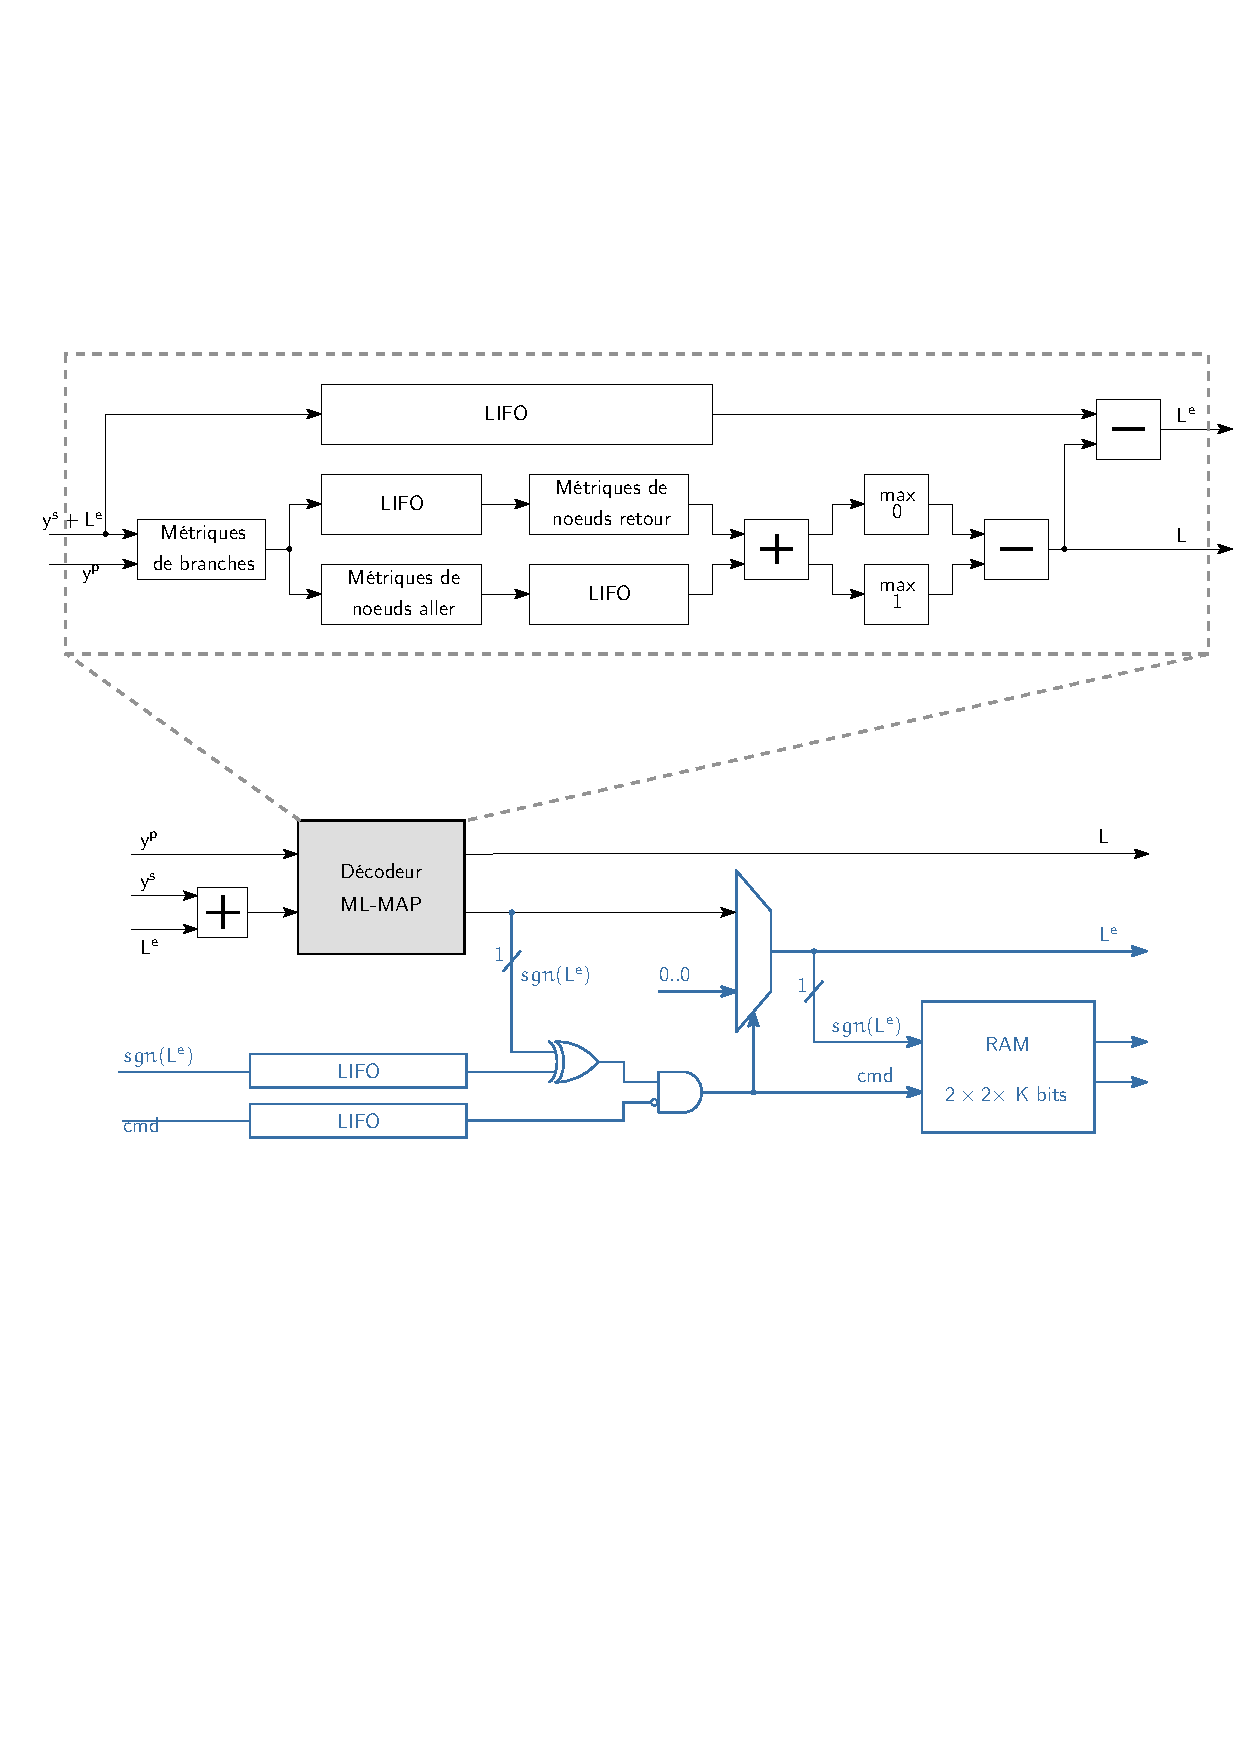
\includegraphics[width=\textwidth]{main/ch2_fig/ipe/sc_arch3.pdf}
	\vspace*{.3cm}
	\caption{\label{fig:sc_arch}Architecture matérielle d'un turbo décodeur séquentiel intégrant le principe Self-Corrected de l'information 
	extrinsèque.}
\end{figure}

Le principe Self-Corrected de l’information extrinsèque doit être réalisé juste avant que l'information extrinsèque ne soit stockée. 
Pour sa mise en œuvre, il est nécessaire d'avoir à disposition deux informations. D'une part, le signe de l'information 
extrinsèque calculée à l'itération précédente et d'autre part la sauvegarde de l'utilisation ou non du principe Self-Corrected à 
l'itération précédente. Ainsi, il est nécessaire de stocker ces deux informations sur deux bits dans une mémoire. Dès lors, 
il suffit de combiner ces deux informations avec le signe de l'information extrinsèque qui vient d'être 
calculée par le décodeur SISO. Le résultat permet de commander un multiplexeur assignant en sortie l'information extrinsèque 
inchangée ou 0.

En résumé l'essentiel de la complexité matérielle introduite par le principe SC consiste en un effort supplémentaire de mémorisation. Par bit 
d'information, deux bits additionnels sont nécessaires. De plus, comme ces deux bits sont 
requis à l'itération suivante et non à la demi-itération suivante, la taille totale de la mémoire additionnelle 
représente $2\times 2 \times 2 \times K$ bits. En comparaison, une architecture séquentielle de turbo décodeur requiert le stockage
de  l'information du canal et de l'information extrinsèque. D'après \cite{livre_declercq}, un choix de quantification 
usuel considère l'utilisation de 6 bits pour l'information provenant du canal et de 7 bits pour l'information extrinsèque.
Il est donc nécessaire de stocker au total $(3\times 6)K + 7 K$ bits. L'effort de mémorisation relatif au bon 
fonctionnement de l'algorithme SC entraîne donc une hausse de 16\% du coût global de mémorisation du décodeur.
La logique combinatoire nécessaire est quant à elle négligeable puisqu'elle
représente un multiplexeur 7 bits, une porte ou-exclusif, une porte inverseuse et une porte et.

Cette architecture peut être adaptée à un parallélisation du décodage. Cela correspond à utiliser plusieurs décodeurs SISO chacun 
travaillant sur une portion de la trame. La taille de la mémoire n'est donc pas modifiée. En revanche, la logique combinatoire
se doit d'être multipliée par le nombre de décodeurs SISO utilisés.
% En revanche, l'adaptation à un décodeur effectuant les calculs en radix-4 
% \cite{radix4} est plus complexe, puisque similaire à un passage à un code double binaire. Néanmoins, ce travail 
% permettrait peut-être de proposer une adaptation du principe Self-Corrected aux turbo codes double-binaires.


\subsection{Conclusions}
Une adaptation de l'algorithme Self-Corrected originellement proposé pour les codes LDPC a été présentée pour les turbo 
codes. Cet algorithme, peu coûteux à mettre en œuvre permet d'obtenir, sans modifier le turbo codeur, des gains dans la zone 
de convergence. Toutefois, cette approche suppose quelques contraintes afin que les gains énoncés soient
 conséquents. D'une part, le nombre maximal d'itérations se doit d'être plus important que dans les schémas de 
 décodage courants. Cependant, grâce à l'utilisation d'un critère d'arrêt, le nombre moyen d'itération employé reste 
 similaire. Ce travail a fait l'objet d'une publication en conférence nationale \citemine{gretsi}.

 D'autre part, afin d'observer des gains aussi en terme de taux d'erreur trame, il est nécessaire que le 
 nombre d'état du codeur soit supérieur à 8. Aucune proposition n'a pu être fournie, quant à la cause de ce phénomène. 
 D'autant plus que les oscillations internes au 
turbo décodeur semblent avoir le même comportement entre 8 et 16 états à la vue des statistiques précédentes. 

Les transpositions au cas des turbo codes double binaire n'ont pas abouti à des gains significatifs. Le faible écart de 
performance entre les algorithmes MAP et ML-MAP dans ce contexte peut expliquer ce résultat.

Finalement, une architecture matérielle compatible avec un décodeur EML-MAP séquentiel a été proposée. Il a été montré 
que l'essentiel du surcoût de complexité matérielle de cet algorithme réside dans la mémorisation. Ce surcoût reste modéré puisque 
seuls $4\times K$ bits supplémentaires sont nécessaires.

\section{Turbo décodages successifs}
Comme évoqué dans le chapitre premier, une approche permettant l'observation de gains de performance à la fois dans la 
zone de convergence et celle du plancher d'erreur est celle reposant sur des décodages multiples. Dans la littérature, trois 
articles majeurs dérivent cette méthode \cite{cim,fsm,pflet}. Dans la suite, le principe de ce type de décodage est rappelé. 
Des performances sont présentées. Une adaptation considérant le nombre d'oscillation comme métrique est enfin présentée.

\subsection{État de l'art : Correction Impulse Method}
L'approche Correction Impulse Method (CIM) est basée sur l'application de turbo décodages successifs. Tout d'abord, un turbo décodage 
classique est réalisé. Si la trame n'est pas corrigée, alors une extraction des positions les moins fiables est effectuée. 
L'extraction est réalisée en prenant en considération les informations \textit{a posteriori} obtenues lors de la dernière 
itération. Plus la valeur absolue de l'information \textit{a posteriori} est faible, moins la décision prise par le 
décodeur est fiable. Une liste de positions non fiables est alors extraite. Tour à tour, la valeur de l'information systématique provenant du canal 
associée aux positions concernées est saturée à une valeur supérieure à la distance minimale du code. Le signe de cette 
valeur de saturation prend le signe opposé au mot obtenu lors du premier turbo décodage. Un nouveau turbo décodage est alors
appliqué. Si le décodage est correct, le processus est stoppé. Sinon, une nouvelle valeur d'information systématique provenant du canal est saturée
et le turbo décodage associé est appliqué. Le nombre maximum de turbo décodage pour une même trame est fixé à 
$L$. L'algorithme \ref{alg:fsm} récapitule l'ensemble de ces opérations.

\begin{center}
\begin{minipage}{.7\textwidth}%
%\vspace*{-.8cm}
% \begin{algorithm}[H]
% \caption{: Correction Impulse Method (CIM)}
% \label{alg:fsm}
% \begin{algorithmic}
% \State $\mathbf{L} \ \ \ \gets \ \ $\Call{Turbo décodage EML-MAP}{}
% \State $\textbf{idx} \gets  \ \ $\Call{Trie selon valeurs croissantes}{L}
% \State \Call{Sauvegarde de $L^s$}{}

% \While{\emph{j} < L et CRC non vérifié }	
% 	\State $L^s[idx[j]] \ \ \ \gets \ \ (-1)^{\hat{d}}\times d_{min}$
% 	\State $\mathbf{L} \ \ \ \gets \ \ $\Call{Turbo décodage EML-MAP}{}
% 	\State \Call{Vérification CRC}{$\mathbf{L}$}
% 	\State \Call{Restauration de $L^s$}{}
% 	\State $j \gets j+1$
% \EndWhile
% \end{algorithmic}
% \end{algorithm}
		\begin{algorithm}[H]
		\DontPrintSemicolon
		%\KwResult{Write here the result }
		\SetKwFunction{TD}{Turbo Décodage EML-MAP}
		\SetKwFunction{ST}{Trie selon valeurs croissantes}
		\SetKwFunction{SA}{Sauvegarde}
		\SetKwFunction{CRC}{CRCheck}
		\SetKwFunction{RT}{Restauration}

		$\mathbf{(L,\hat{d})} \gets$ \TD{$\mathbf{y^s,\ y^{p},\ y^{'p}}$}\;
		$\mathbf{idx} \gets$ \ST{$\mathbf{L}$}\;
		\SA{$\mathbf{y^s}$}\;
		$j \gets 0$\;
		\While{$j<L$ et \CRC{$\mathbf{\hat{d'}}$}==false}{
			\RT{$\mathbf{y^s}$}\;
			$\mathbf{y^s}\left[\mathbf{idx}[j]\right] \gets \ (-1)^{\hat{d}}\times d_{min}$\;
			$\mathbf{\hat{d'}} \gets$ \TD{$\mathbf{y^s,\ y^{p},\ y^{'p}}$}\;
			$j\gets j+1$\;
		}
	\caption{: Correction Impulse Method (CIM)}
	\label{alg:fsm}
	\end{algorithm}
\end{minipage}
\end{center}

L'amplitude de la saturation est choisie de telle sorte qu'elle soit supérieure à $d_{min}$ pour s'assurer que le décodeur 
fournisse un résultat différent du premier. Ceci est à mettre en corrélation avec la méthode d'obtention de la distance 
minimale d'un turbo code par la méthode d'impulsion d'erreur \cite{eim} présentée dans le premier chapitre.

Dans \cite{cim}, les turbo codes double binaires sont aussi considérés. Pour chaque symbole, 4 valeurs LLR \textit{a 
posteriori} sont générées. La métrique permettant d'identifier les positions les moins fiables consiste alors à prendre 
la différence entre la plus grande valeur de LLR et la deuxième plus grande valeur de LLR. Trois turbo décodages sont 
réalisés pour chaque position identifiée. Ainsi, les trois sens de saturation associés aux trois autres symboles possibles 
en excluant le symbole décodé sont considérés. Le nombre maximal de turbo décodages vaut alors $3\times L + 1$.

Dans cette publication, des simulations ayant pour cadre des turbo codes binaire et double binaires à 8 états, de 
rendement 1/3 et 1/2 et avec une taille d'information binaire de 1504 bits. L'algorithme EML-MAP itérant au maximum 16 fois est
employé. Plusieurs nombres de décodages supplémentaires sont considérés, allant de 1 à la taille de la trame. Dans tous 
les cas, des gains dans les zone de convergence apparaissent, augmentant avec $L$. Cependant, les gains les plus significatifs
se trouvent dans la zone du plancher d'erreur. Dans le cas binaire, avec $L=1$, les gains atteignent un ordre de grandeur. 
La multiplication par 4 de L permet à chaque fois d'augmenter les gains d'environ un ordre de magnitude.\\
Dans le cas double binaire, les gains globaux sont moins important mais dépassent tout de même un ordre de magnitude 
avec $L=4$. 

Dans \cite{fsm}, il est montré qu'une amélioration des performances est observée lorsque tous les sens de 
saturation sont testés. Ainsi, dans le cas binaire, deux turbo décodages sont effectués par position identifiée. Pour 
un turbo code double binaire, 4 turbo décodages peuvent être réalisés successivement. Dans cette publication, des 
simulations sont présentées pour un turbo code double binaire à 8 états et de rendement 1/2. La taille de trame est 
de 1504. Dans performances similaires à celles de \cite{cim} sont observées. Cette approche est nommée
Forced Symbol Method (FSM).

Finalement, \cite{pflet} étend le principe de turbo décodages successifs en considérant cette fois l'ensemble des positions de la trame ($1/R\times K$). 
Ainsi, au maximum, $2\times 1/R\times K$ turbo décodages peuvent être réalisés pour une trame. Les informations
de redondance provenant du canal peuvent être elles aussi saturées. Cette approche permet donc d'aboutir aux meilleures
performances de décodage grâce au principe de turbo décodages successifs. De part son contexte ne nécessitant pas toujours 
une forte contrainte en latence, le standard CCSDS est choisi comme cadre d'étude. À l'inflexion entre la zone de convergence 
et celle du plancher d'erreur, cet algorithme permet d'obtenir un 
gain de deux ordres de magnitude faisant passer le taux d'erreur trame d'environ $10^{-6}$ à $10^{-8}$. En adjonction du 
FSM, un décodage de Viterbi par liste est aussi considéré. Cependant, les auteurs indiquent que 
le gain de performance amené par ce second algorithme est marginal. Finalement, les auteurs statuent sur 
le fait qu'un code CRC de taille 16 ou moins est restrictif dans cette approche puisque la probabilité d'erreur non 
détectée devient trop importante. Dans \cite{fsm}, les auteurs considèrent qu'un code CRC de taille 24 est suffisant pour 
que l'approche de turbo décodages successifs ne soit pas impactée par le code CRC.

\begin{figure}[!h]
	\centering
	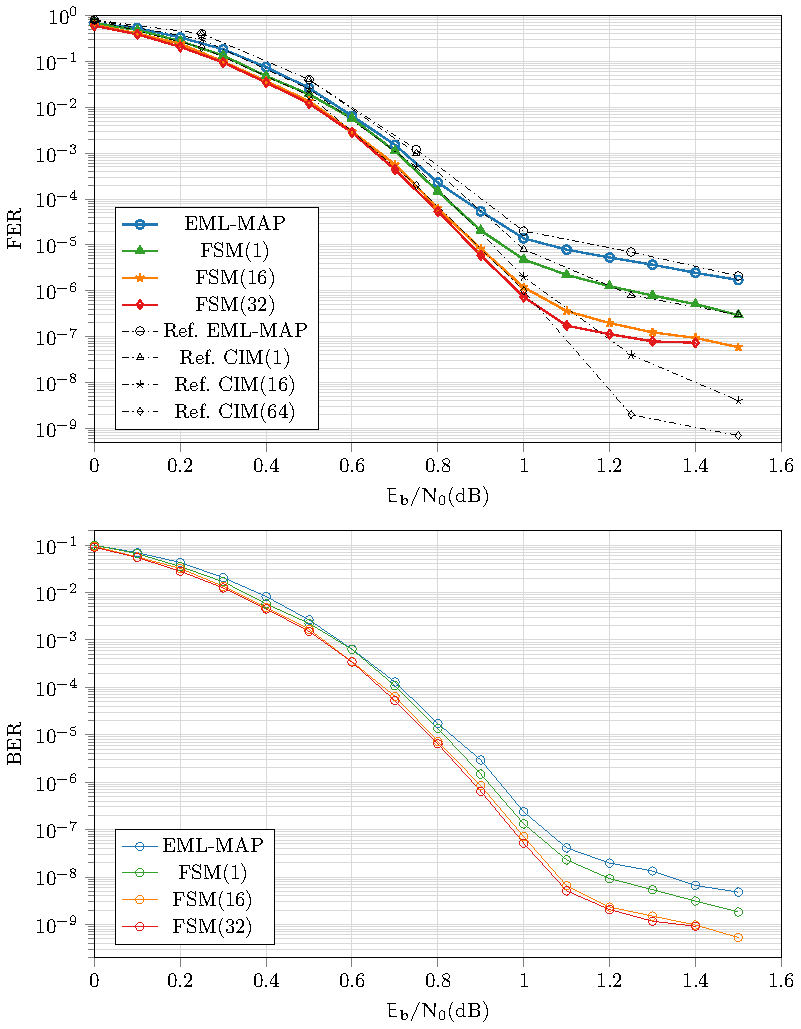
\includegraphics[width=.8\textwidth]{main/ch2_fig/tikz/redec_fsm.pdf}
	\vspace*{.3cm}
	\caption{\label{fig:fsm}Comparaison des performances de décodage entre les algorithme EML-MAP et FSM avec plusieurs 
	profondeurs de recherche. Turbo code du standard LTE (K=1504, R=1/3).}
\end{figure}

La Figure \ref{fig:fsm} (a) présente les taux d'erreur trame relevés dans \cite{cim} dans le cadre d'un turbo code binaire,
de rendement 1/3 et de taille de trame 1504. Un entrelaceur DRP (cf. \ref{sec:entrelacement})  est utilisé. Chaque processus de turbo décodage itère 
jusqu'à 16 fois. La notation CIM(L) signifie qu'au maximum L différentes positions dans la trame peuvent être saturées. 
Ces différentes courbes sont présentées en pointillé.

Une reproduction des résultats a été tentée. Cependant, les paramètres de l'entrelaceur DRP ne sont pas fournis. 
L'entrelaceur LTE a alors été utilisé. Ce dernier est basé sur une permutation QPP. Les propriétés de distance du turbo 
code résultant sont donc normalement aussi bonnes que celles obtenues avec l'entrelaceur DRP. Dans \cite{cim}, un critère 
d'arrêt génie est considéré. Afin de statuer sur un système réaliste, le code CRC du standard LTE est utilisé comme 
critère d'arrêt. Enfin, dernière différence dans cette tentative de reproduction des résultats, le turbo décodeur peut 
itérer au maximum 32 fois. C'est pourquoi un léger avantage dans la zone de convergence apparaît mais cette augmentation du nombre 
d'itérations n'a pas d'impact sur la zone du plancher d'erreur puisque elle dépend principalement des propriétés 
de distance du code.

Sans turbo décodages successifs, les performances de décodage sont semblables. Un léger gain en convergence apparaît 
sur  la courbe pleine provenant de l'augmentation du nombre d'itérations. En considérant $L=1$, les performances dans la
zone du plancher d'erreur sont à nouveau similaires. Cependant, la référence considère un seul sens de saturation par position
retenue alors que l'approche FSM(1) en considère deux. 

Lorsque l'identification des 16 positions les moins fiables est appliquée, pour une valeur de SNR inférieure à 1.1 dB, les 
performances de décodage sont similaires. En revanche dans la tentative de reproduction des résultats, la zone du plancher
d'erreur arrive dès 1.2 dB alors que dans \cite{cim}, l'inflexion de la courbe est bien moins marquée permettant à ce 
schéma de décodage d'atteindre un FER de $4.10^{-9}$ pour une valeur de SNR de 1.5 dB alors qu'elle n'est que de $8.10^{-8}$
dans notre cas. Si la valeur de $L$ augmente, des résultats similaires sont observés. Pour la référence, 
l'inflexion diminue, le plancher d'erreur se voit dramatiquement abaissée fournissant des gains importants en utilisant
cette méthode. Cependant, dans notre tentative de reproduction des résultats ce comportement n’apparaît pas, la zone du 
plancher d'erreur se trouvant être dans la plage de taux d'erreur $[10^{-8}~;~10^{-7}]$. Plusieurs valeurs de saturation 
ont aussi été considérées, sans succès sur l'amélioration des performances :
\begin{itemize}
	\item 0.0, correspondant à une annulation de la contribution, 
	\item 4.0, correspondant à une faible saturation du décodeur. Cette valeur est similaires à celles obtenues en sortie du canal,
	\item 10.0, correspondant environ à la moitié de la distance minimale du code,
	\item 25.0, correspondant environ à la distance minimale du code, comme préconisé dans \cite{cim, fsm},
	\item 35.0, correspondant à une valeur supérieure à la $d_{min}$, assurant, normalement un décodage différent.
\end{itemize}
Aucune de ces valeurs n'a permis d'aboutir à un comportement réellement différent au niveau des simulations Monte-Carlo.

Les résultats en terme de taux binaire sont quant à eux difficiles à analyser. En effet, les simulation Monte-Carlo 
ont été réalisées de telle sorte que si le code CRC n'est pas vérifié, la trame produite par le décodeur est la dernière calculée.
Or, celle-ci correspond à la trame avec l'impulsion localisée sur la position la plus fiable parmi celles considérées. 
Il en résulte que si la trame n'est pas corrigée une augmentation du nombre d'erreurs dans la trame erronée apparaît. Ainsi, 
si le code CRC n'est pas vérifié, afin d'obtenir les meilleurs performances en taux d'erreurs trame et binaire, il faudrait 
transmettre le mot obtenu à l'issue du premier décodage.

Plusieurs explications peuvent expliquer la différence des résultats en terme de taux d'erreur trame. Tout 
d'abord,  dans \cite{cim}, l'impact de la méthode est évalué pour un sous ensemble de trames erronées à l'issue du premier 
décodage. Ainsi, les taux d'erreur calculés risquent de ne pas être statistiquement stables. \\
D'autre part, l'entrelaceur peut aussi avoir un impact important.
En effet, il est conjecturé dans \cite{fsm} que cette méthode permet, grâce à l'utilisation du CRC, d'augmenter la distance
minimale du code. Ainsi, au niveau du spectre de distance du code, cela revient à supprimer au moins son premier terme.
Les distance minimales obtenues via les différents formalismes d'entrelaceurs courants (DRP, QPP et ARP) sont équivalentes. 
Ceci est vérifié par le fait que les courbes de la Figure \ref{fig:fsm} sont semblables avec un décodage 
EML-MAP. En revanche, entre deux entrelaceurs permettant d'atteindre la même distance minimale (ayant le plus grand impact
sur la zone du plancher d'erreur), les termes suivants du spectre peuvent différer. Si la distance entre les deux 
premières valeurs du spectre de distance est plus importante pour l'entrelaceur DRP considéré que pour l'entrelaceur LTE, alors la 
suppression du premier terme augmente d'autant plus l'abaissement du plancher d'erreur. Malheureusement cette explication ne 
peut être vérifiée qu'avec l'obtention des paramètres de l'entrelaceur DRP utilisé dans \cite{cim}.\\
Finalement, la dernière explication pouvant être conjecturé est la limitation induite par les capacités de détection du
code CRC considéré. Cependant, il est indiqué dans \cite{fsm} qu'un code CRC de taille 24 devrait être suffisante. Ainsi, 
des tests incluant l'utilisation d'un critère d'arrêt génie ont été réalisés. Des gains ont été observés sans toutefois 
permettre de reproduire les performances présentées dans \cite{cim}.

Pour conclure sur ces techniques utilisant des décodages successifs, malgré les différentes configuration testées, les 
gains énoncés dans la zone du plancher d'erreur n'ont pu être reproduits. Des gains sont observés mais ils 
dépassent difficilement un ordre de magnitude dans le plancher d'erreur. En revanche, dans la zone de convergence, les gains 
constatés sont similaires. 
% Finalement, \cite{pflet} a pour cadre le turbo code du standard CCSDS. Ainsi, les paramètres de l'entrelaceur sont disponibles
%aisément. Cependant, seules les performances dans la zone de convergence sont présentées, ne permettant pas de statuer sur
%la zone du plancher d'erreur.

Néanmoins, le principe de décodage successif est attrayant car relativement facile à mettre en œuvre pour une implémentation logicielle.
Pour pour des communications ayant une faible contrainte de latence, ce principe permet d'apporter une solution relativement
simple pour abaisser le plancher d'erreur. 
Dans la section suivante, une métrique basée sur les oscillations au sein du turbo décodeur est alors proposée. Les performances
résultantes sont comparées avec les performances présentées dans cette section.

\subsection{Utilisation de métriques basée sur les oscillations}
La Section \ref{sec:observ} a mis en exergue une corrélation entre le nombre d'erreurs à l'issu du décodage et 
le nombre d'oscillations durant le processus itératif. Ainsi, la proposition faite dans cette section en découle. Elle 
consiste à identifier les positions dans la trame qui ont le plus oscillé avant de réaliser, à partir de cette liste, des turbo décodages successifs.

En effet, il parait intuitif de statuer que saturer l'information du canal d'un bit oscillant fortement lors du 
premier décodage va fondamentalement modifier le résultat produit par le turbo décodeur. Ainsi, l'algorithme \ref{alg:fsm}
n'est que peu modifié. Durant le premier turbo décodage, en plus de fournir la trame décodée, le décodeur doit produire le 
nombre d'oscillations recensées pour chacun des bits durant le processus itératif. Cette information est alors triée 
selon un ordre décroissant. Les index associés aux bits ayant les plus oscillé sont alors pris en compte pour modifier 
l'information du canal avant d'effectuer des turbo décodage successifs. L'algorithme \ref{alg:osc} récapitule ces différentes 
étapes.
\begin{center}
\begin{minipage}{.9\textwidth}%
% \begin{algorithm}[H]
% \caption{: Forced Symbol Method, identification sur oscillation (OFSM)}
% \label{alg:osc}
% \begin{algorithmic}
% \State $\mathbf{L, osc} \ \ \ \gets \ \ $\Call{Turbo décodage EML-MAP}{}
% \State $\textbf{idx} \gets  \ \ $\Call{Trie des bits selon valeurs décroissantes}{osc}
% \State \Call{Sauvegarde de $L^s$}{}
% \While{\emph{j} $< 2\times L$ et CRC non vérifié }	
% 	\State $L^s[idx[j]] \ \ \ \gets \ \ (-1)^{j\mod{2}}\times d_{min}$
% 	\State $\mathbf{L} \ \ \ \gets \ \ $\Call{Turbo décodage EML-MAP}{}
% 	\State \Call{Vérification CRC}{$\mathbf{L}$}
% 	\State \Call{Restauration de $L^s$}{}
% 	\State $j \gets j+1$
% \EndWhile
% \end{algorithmic}
% \end{algorithm}
	\begin{algorithm}[H]
		\DontPrintSemicolon
		%\KwResult{Write here the result }
		\SetKwFunction{TD}{Turbo Décodage EML-MAP}
		\SetKwFunction{ST}{Trie selon valeurs decroissantes}
		\SetKwFunction{SA}{Sauvegarde}
		\SetKwFunction{CRC}{CRCheck}
		\SetKwFunction{RT}{Restauration}

		$\mathbf{(L,\hat{d},osc)} \gets$ \TD{$\mathbf{y^s,\ y^{p},\ y^{'p}}$}\;
		$\mathbf{idx} \gets$ \ST{$\mathbf{osc}$}\;
		\SA{$\mathbf{y^s}$}\;
		$j \gets 0$\;
		\While{$j<2\times L$ et \CRC{$\mathbf{\hat{d'}}$}==false}{
			\RT{$\mathbf{y^s}$}\;
			$\mathbf{y^s}\left[\mathbf{idx}[j]\right] \gets \ (-1)^{j {~mod~} 2} \times d_{min}$\;
			$\mathbf{\hat{d'}} \gets$ \TD{$\mathbf{y^s,\ y^{p},\ y^{'p}}$}\;
			$j\gets j+1$\;
		}
	\caption{: Forced Symbol Method, identification sur oscillation (OFSM)}
	\label{alg:osc}
	\end{algorithm}
\end{minipage}
\end{center}

Le comportement des oscillations diffère selon un décodage basé sur l'algorithme EML-MAP ou sur l'algorithme ML-MAP. En effet, 
l'introduction d'un facteur d'échelle réduit l'amplitude des valeurs de l'information extrinsèque. Ceci permet d'atténuer 
l'avis du décodeur et donc de réduire son impact sur le décodage à la demi-itération suivante. Ceci a pour effet de 
réduire les oscillations puisque le poids des information calculées à la demi-itération précédente est lui même réduit. 
Ainsi, l'algorithme EML-MAP possède de meilleures performances de base que l'algorithme ML-MAP. Cependant, la réduction 
des oscillations au sein du processus itératif a pour effet de rendre moins discrétisant la métrique induite 
précédemment.

\begin{figure}[!h]
	\centering
	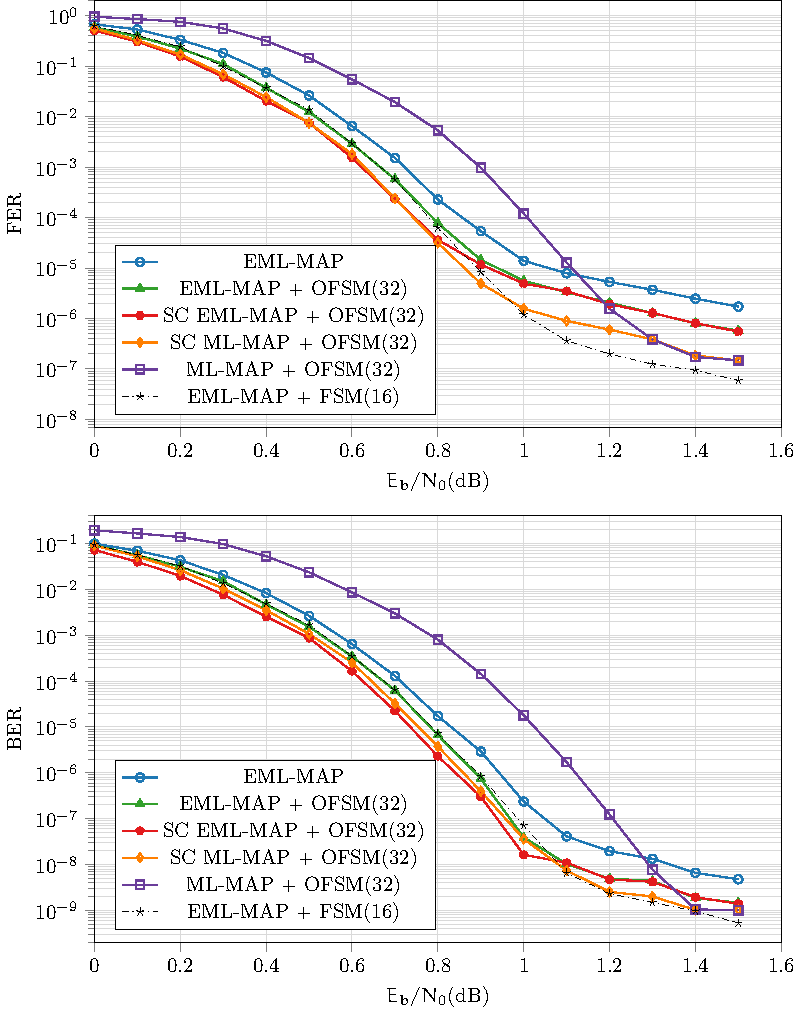
\includegraphics[width=.8\textwidth]{main/ch2_fig/tikz/redec_osc.pdf}
	\vspace*{.3cm}
	\caption{\label{fig:cmp_osc}Comparaison des performances de décodage entre les algorithme EML-MAP et FSM pour plusieurs 
	profondeurs de recherche. Turbo code du standard LTE (K=1504, R=1/3).}
\end{figure}

La Figure \ref{fig:cmp_osc} présente les performances de décodage obtenues en exploitant le principe de décodages successifs selon une 
métrique basée sur le nombre d'oscillations. Un turbo code du standard LTE est considéré avec des paquets de 1504 bits et un 
rendement 1/3. Chaque turbo décodage peut effectuer jusqu'à 32 itérations. La notation OFSM(L) signifie qu'au plus L 
positions différentes seront saturées dans les deux directions. Différents algorithmes sont utilisés au sein du
processus itératif. Sont considérés les algorithmes 
\begin{itemize}
 	\item EML-MAP,
 	\item SC EML-MAP,
 	\item ML-MAP et 
 	\item SC ML-MAP.
 \end{itemize} 
 Ainsi, il s'agit de l'algorithme 
max-log-MAP avec ou sans remise à l'échelle et avec ou sans principe Self-Corrected de l'information extrinsèque.

Lorsque l'algorithme EML-MAP est employé, les décodages successifs permettent un léger gain dans la zone de convergence 
et dans la zone du plancher d'erreur. Ce gain correspond à un facteur 3. Si maintenant l'algorithme SC EML-MAP 
est  choisi, une nouvelle amélioration dans la zone de convergence apparaît. Celle-ci correspond au gain apporté par le 
principe Self-Correct de l'information extrinsèque au premier décodage. Si maintenant la remise à l'échelle n'est plus 
considérée (algorithme SC ML-MAP), alors les gains sont constants dans la zone de convergence. En revanche, ils augmentent dans 
la zone du plancher d'erreur. Ainsi, des gains à la fois dans la zone de convergence et dans le plancher d'erreur 
approchent l'ordre de grandeur. Finalement,sans modification de l'information extrinsèque 
(algorithme ML-MAP), une retard important sur le seuil de converge apparaît. Celui-ci représente presque 0.2 dB en terme 
de valeur de SNR. En revanche, cette courbe de performance rejoint celle obtenue avec le principe SC dans la zone du 
plancher d'erreur. 

Toutefois, les performances obtenues avec l'algorithme FSM(16) sont proches voire meilleures. C'est pourquoi l'approche 
d'identification par les oscillations seules n'apporte pas de gains suffisants par rapport à l'état de l'art.

\section{Conclusions}
Dans ce deuxième chapitre, une étude des oscillations internes au processus de décodage itératif des turbo codes a été 
menée. Dans un premier temps, des observations statistiques ont permis d'observer de fortes corrélations entre des oscillations
et des erreurs. Cependant, il n'y a pas pour autant d'implication entre ces oscillations et les erreur. Cette dernière constatation 
rend délicat une possibilité d'identification de la position des erreurs grâce à l'observation des oscillations.

Cependant, une utilisation de cette observation est proposée afin de corriger l'information extrinsèque échangée au 
cours du processus itératif. L'algorithme résultant a été proposé pour les turbo codes binaires, aucune adaptation intéressante 
pour les turbo codes double binaires n'a pu être trouvé. Dans le cas binaire, sous couvert d'un nombre maximal d'itération
important, le seuil de convergence apparaît plus vite qu'avec l'algorithme EML-MAP fonctionnant avec le même nombre 
d'itérations. Des gains de décodage ont été obtenus dans le cadre du standard CCSDS, représentant un ordre de grandeur en terme de taux d'erreur trame 
ou 0.1 dB de gain pour la valeur de SNR. Une architecture matérielle a été proposée afin de démontrer le faible surcoût au niveau de la complexité
calculatoire.

Finalement, les oscillations ont été étudiées en tant que métrique permettant l'activation de décodages successifs. 
Cependant, aucun gain conséquent n'a pu être observé. Dans le chapitre suivant, une proposition d'algorithme se servant de 
 principes connexes à ceux utilisés dans le cadre des décodage successifs est faite. Ce dernière aboutit à une réduction
du plancher d'erreur sans utiliser de décodage souple supplémentaire.